\documentclass[../../main.tex]{subfiles}

 \lhead{Implementation: Odeon}
 
\begin{document}

\subsection{ODEON}
	\label{odeon}
	\subsubsection{Water Tightness Test}
		Once the SketchUp model had been exported as a .par file using the SU2Odeon plug-in \cite{SU2Odeon} it could be opened in Odeon and checked to ensure that there were no gaps in the model for which rays to escape. If this was the case, the model would have to be fixed in SketchUp and reimported into Odeon. Odeon makes checking the model easy by running a `\textbf{water tightness}' check where a large number of rays are reflected around the room seeing whether any of them manage to escape. Figure~\ref{watertight} shows the Hendrix Hall model undergoing such a test. Once it was ensured that the model was fit for use, the surface materials could be assigned.

		%-------------Water tightness test-------------%
		\begin{figure}[H]
			\center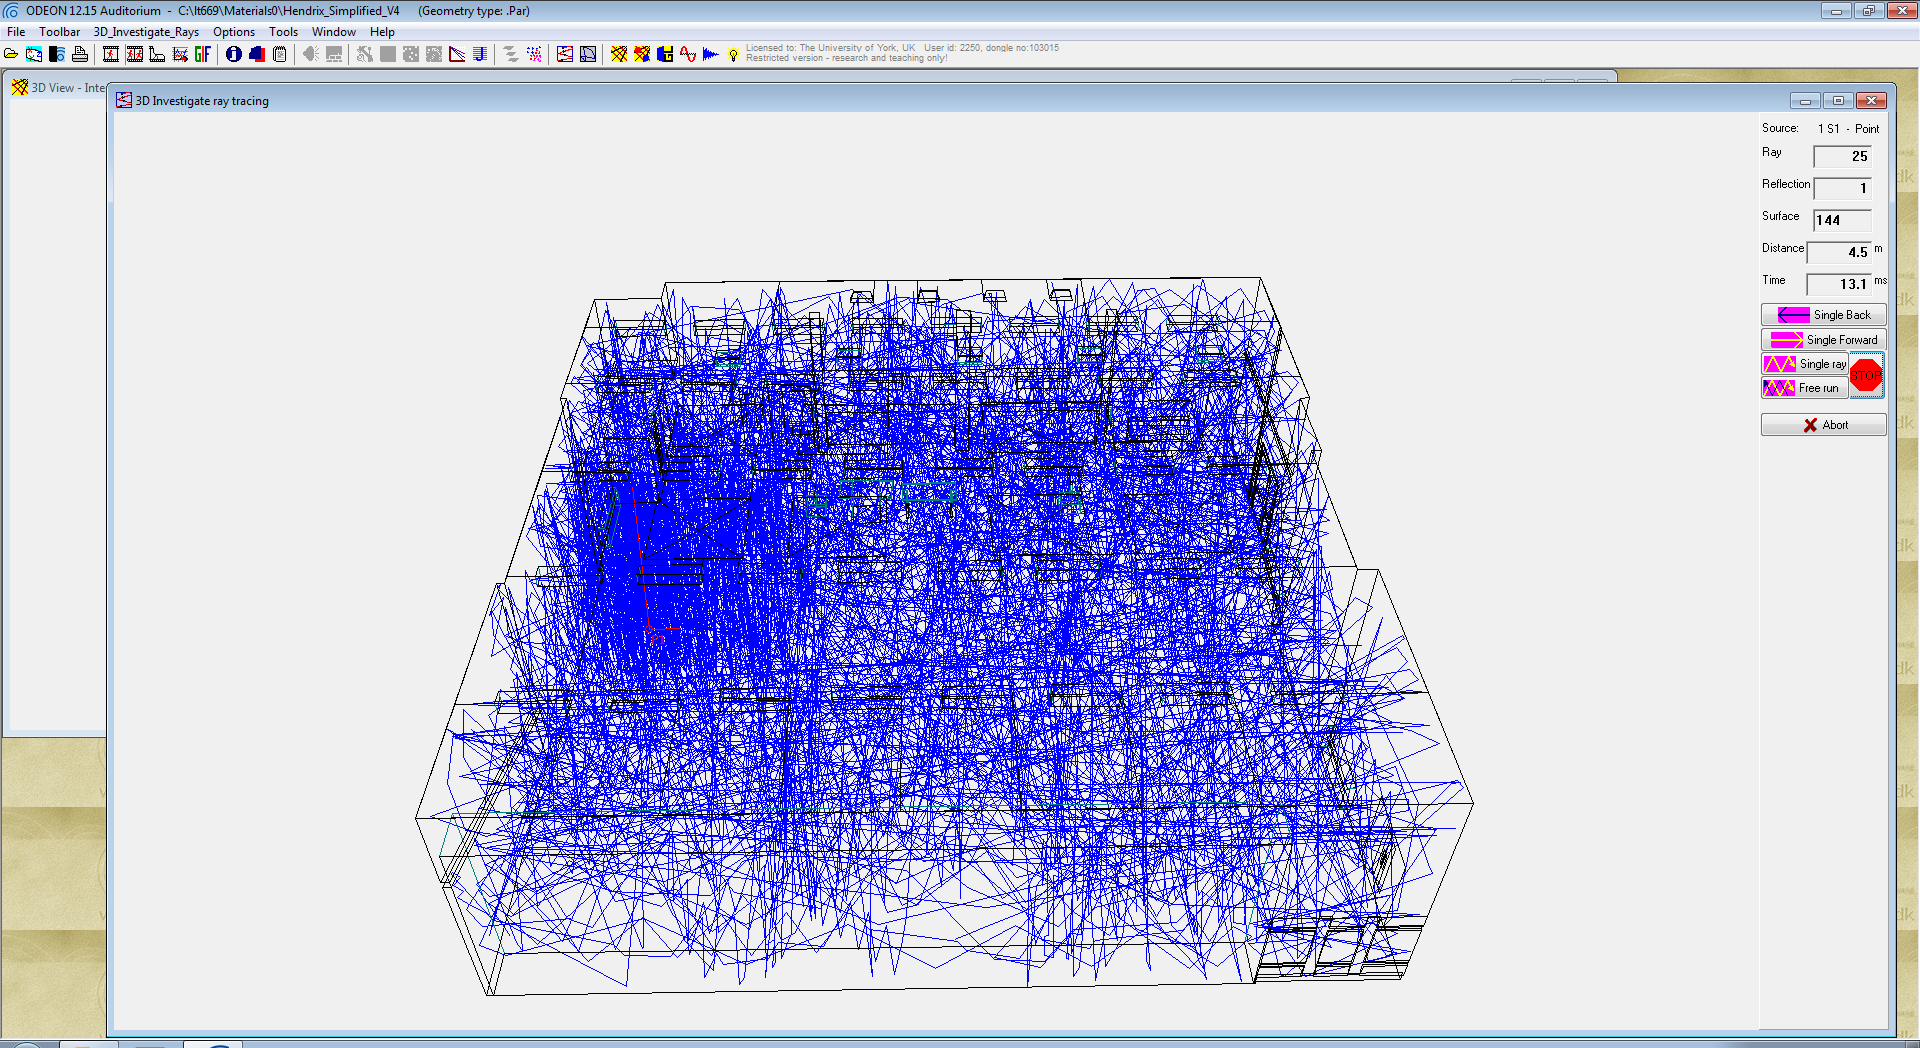
\includegraphics[scale = 0.3]{Sections/Implementation/Odeon/images/OdeonRays/waterTight2.PNG}
			\caption{Hendrix Hall model undergoing a water tightness test in Odeon.}
			\label{watertight}
		\end{figure}

	\subsubsection{Material Selection}
	\label{odeon:materials}
		The surface materials within a room heavily influence how sound propagates around a room, effecting reverberation time and frequency content of said reverb. It is therefore imperative to assign materials as close to the real material as possible in order to produce an accurate representation of a known acoustic environment. For this, Odeon provides a list of common materials often found when constructing buildings.

		\paragraph{Initial Materials}

			Odeon's material list appears to be designed for auralisation of structures with very basic interior. Due to a lack of choice, exact materials in the room could not be modelled accurately, however the closest match to what is thought to be the true material was selected as a replacement instead. In some cases, appropriate replacement materials were not available, therefore new materials had to be added to the material list. This can be done by finding a materials absorption coefficients, selecting `\textbf{Edit an existing material}' where new materials absorption coefficients can be entered and saved as a new material as shown in figure~\ref{materialEdit}. Absorption coefficient values range from 0 - 1 (0\% - 100\%), indicating the percentage of attenuation applied to the selected frequency band upon a contact with the surface. Required materials for which an appropriate replacement could not be found in the material list are listed in table~\ref{materialTable}.

			\begin{table}[H]
			\begin{center}
				\begin{tabular}{r l}
					\textbf{Material} & \textbf{Surface applied to} \\ \hline
					Hard Plastic \cite{plastic} & Roof lights and projector covers \\
					Mineral fibre \cite{mineralFibre} & Ceiling Tiles \\
					Slate \footnotemark[1] \cite{Kovalchik} & Blackboard \\
				\end{tabular}
			\end{center}
			\caption{Table of materials for which absorption coefficients were sought and added to Odeon's material list.}
			\label{materialTable}
			\end{table}

			%-------------Footnote-------------%			
			\footnotetext[1]{The absorption coefficients provided were only available for the 125Hz to 4kHz octave bands, therefore absorption coefficients for the 63Hz and 8kHz octave bands were given a value of 0.1}

			%-------------Material Edit Image-------------%
			\begin{figure}[H]
				\center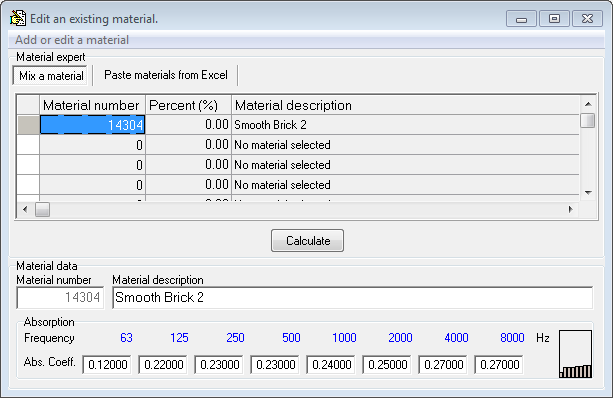
\includegraphics[scale = 0.6]{Sections/Implementation/Odeon/images/Absorption.PNG}
				\caption{Absorption coefficient editing window in Odeon used to add unavailable materials.}
				\label{materialEdit}
			\end{figure}

		\paragraph{Surface Types}

			For a number of surfaces it is appropriate to edit properties other than just their absorption coefficients. As explained in section \nameref{designRoom}, the roof hangings are constructed of four joint slanting surfaces. By changing the individual surface types from \textbf{`Normal'} to \textbf{`Fractional'}, Odeon avoids erroneously calculating the diffraction caused due to each of the individual surfaces and treats them as a whole surface. For surfaces such as the contracted seating shown in figure~\ref{seating} where gaps are present in the over all structure, it was possible to model this as one solid object and to set a \textbf{transparency} value. A transparency value of 0 means the surface is a solid where as a value of 1 makes a surface totally transparent which will let ways pass straight through. A transparency value of 0.3 was chosen as a reasonable estimate, the effects of which are shown in figure~\ref{transparency}, showing how a ray can pass through the front of the object, propagate around the inside and eventually reflect back out again.


				%-------------Seating Image-------------%
			\begin{figure}[H]
				\center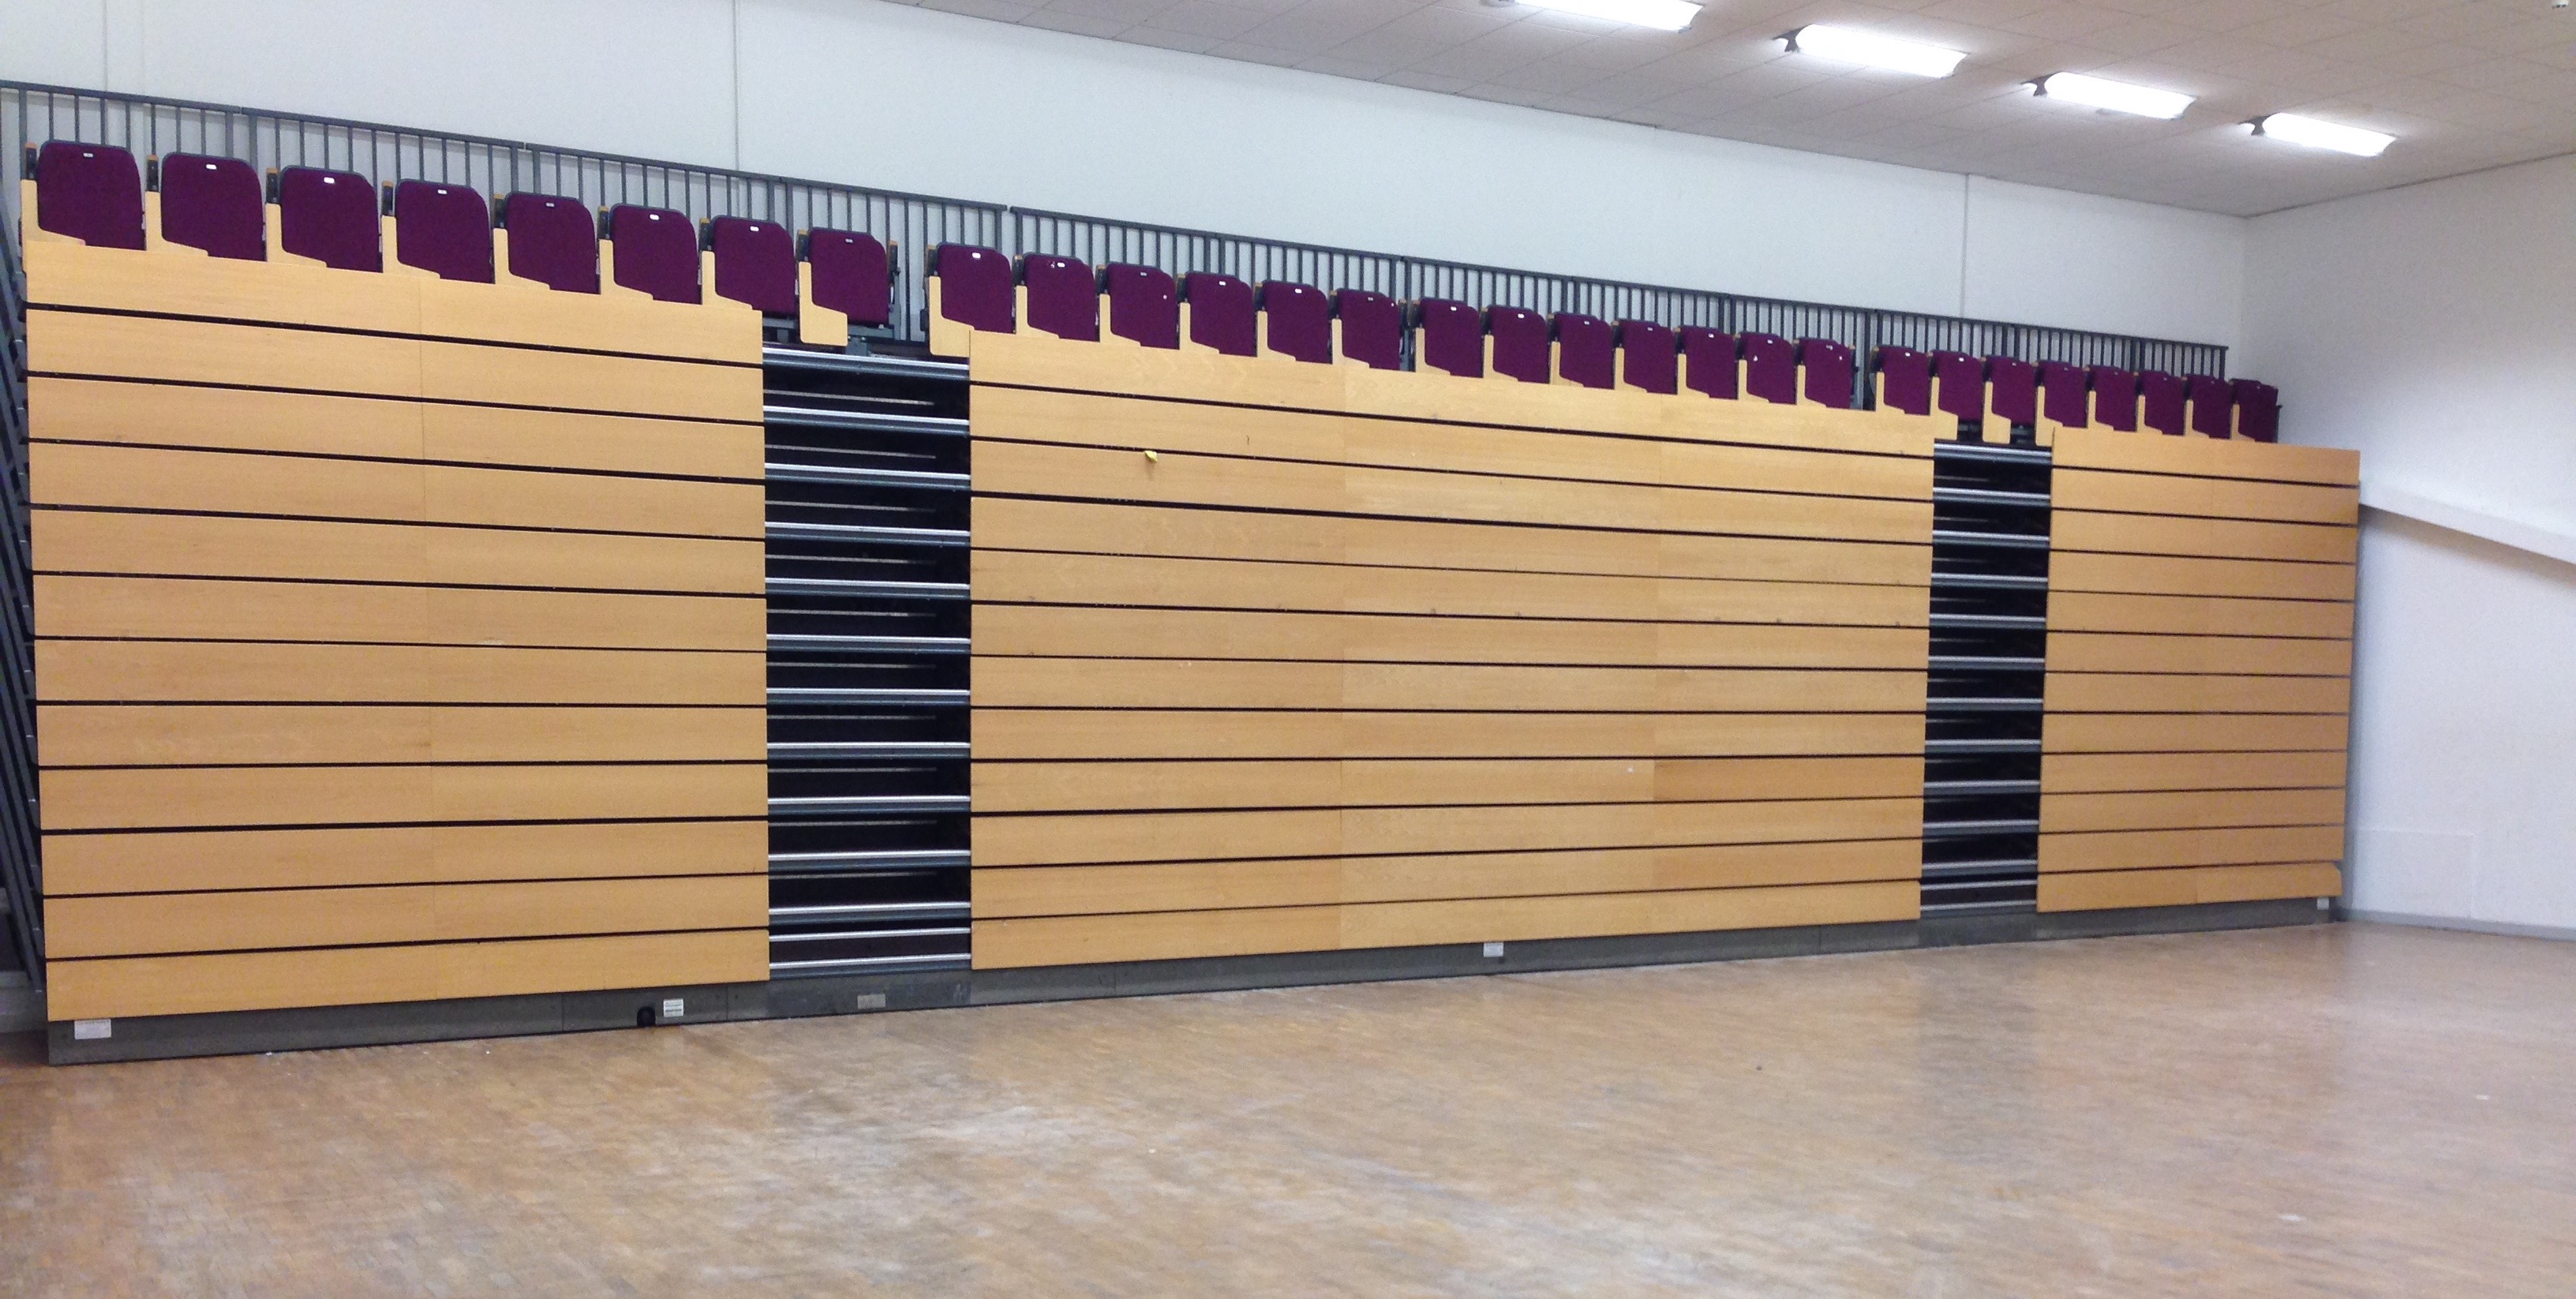
\includegraphics[scale = 0.12]{Sections/Implementation/Odeon/images/seating.jpg}
				\caption{Contracted seating in Hendrix Hall showing gaps in the structure.}
				\label{seating}
			\end{figure}

			%-------------Transparency Image-------------%
			\begin{figure}[H]
				\center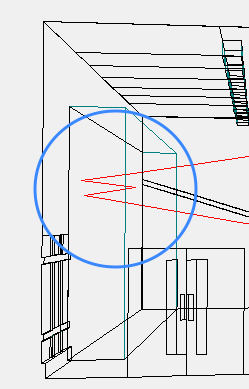
\includegraphics[scale = 0.7]{Sections/Implementation/Odeon/images/OdeonRays/transparencyEdit/singleRay2_edit3.PNG}
				\caption{Blue circle highlights a ray penetrating the modelled seating area, reflecting 3 times and escaping the seating area due to the transparency value set.}
				\label{transparency}
			\end{figure}

			As previously mentioned in section~\nameref{designRoom}, the lights were modelled as simple rectangles as opposed to the more complex objects made from a large number of surfaces with the intention of more accurately modelling the scattering effect (descripbed in section~\nameref{background:scattering}) due to their shape by altering the objects \textbf{Scattering Coefficient}. Odeon provides a table of initial indicators for possible scattering coefficients, shown in figure~\ref{odeonTable} which can be used to select the scattering coefficient for a surface that fits a similar description to the one given. A scattering coefficient of 0.2 was selected for the lights by assuming the effect would not be as sever as a bookshelf. \textbf{[Seriously, re-word this bit]}.

			%-------------Scattering Coefficients table-------------%
			\begin{figure}[H]
				\center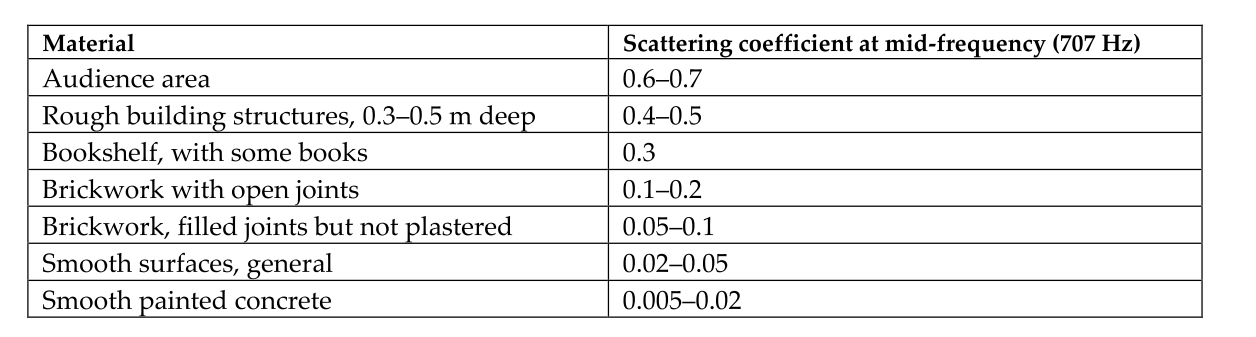
\includegraphics[scale = 0.3]{Sections/Implementation/Odeon/images/scatteringCoefficients.png}
				\caption{A table provided in the Odeon Manual \cite{odeonManual} that can be used to set an approximate scattering coefficient for surfaces similar to those described}
				\label{odeonTable}
			\end{figure}
		
		\paragraph{RIR Comparison}

			Once the initial materials had been selected, the authenticity of the \ac{RIR}'s were checked by comparing their frequency content against that of a real measured \ac{RIR} from Hendrix Hall (see section~\nameref{realRIRs}). This was done by using Matlab to plotting the spectrograms of the omni-directional W channel of both \ac{RIR}'s, as can be seen in figure~\ref{compareOriginal}. The spectrogram shows the high frequency content in the real \ac{RIR} attenuating in a smooth roll off fashion from 20kHz to about 8kHz starting from about 0.2 seconds in, where as the full audible spectrum appears to attenuate almost evenly in the Odeon produced \ac{RIR}.

			%-------------Original materials compare-------------%
			\begin{figure}[H]
				\center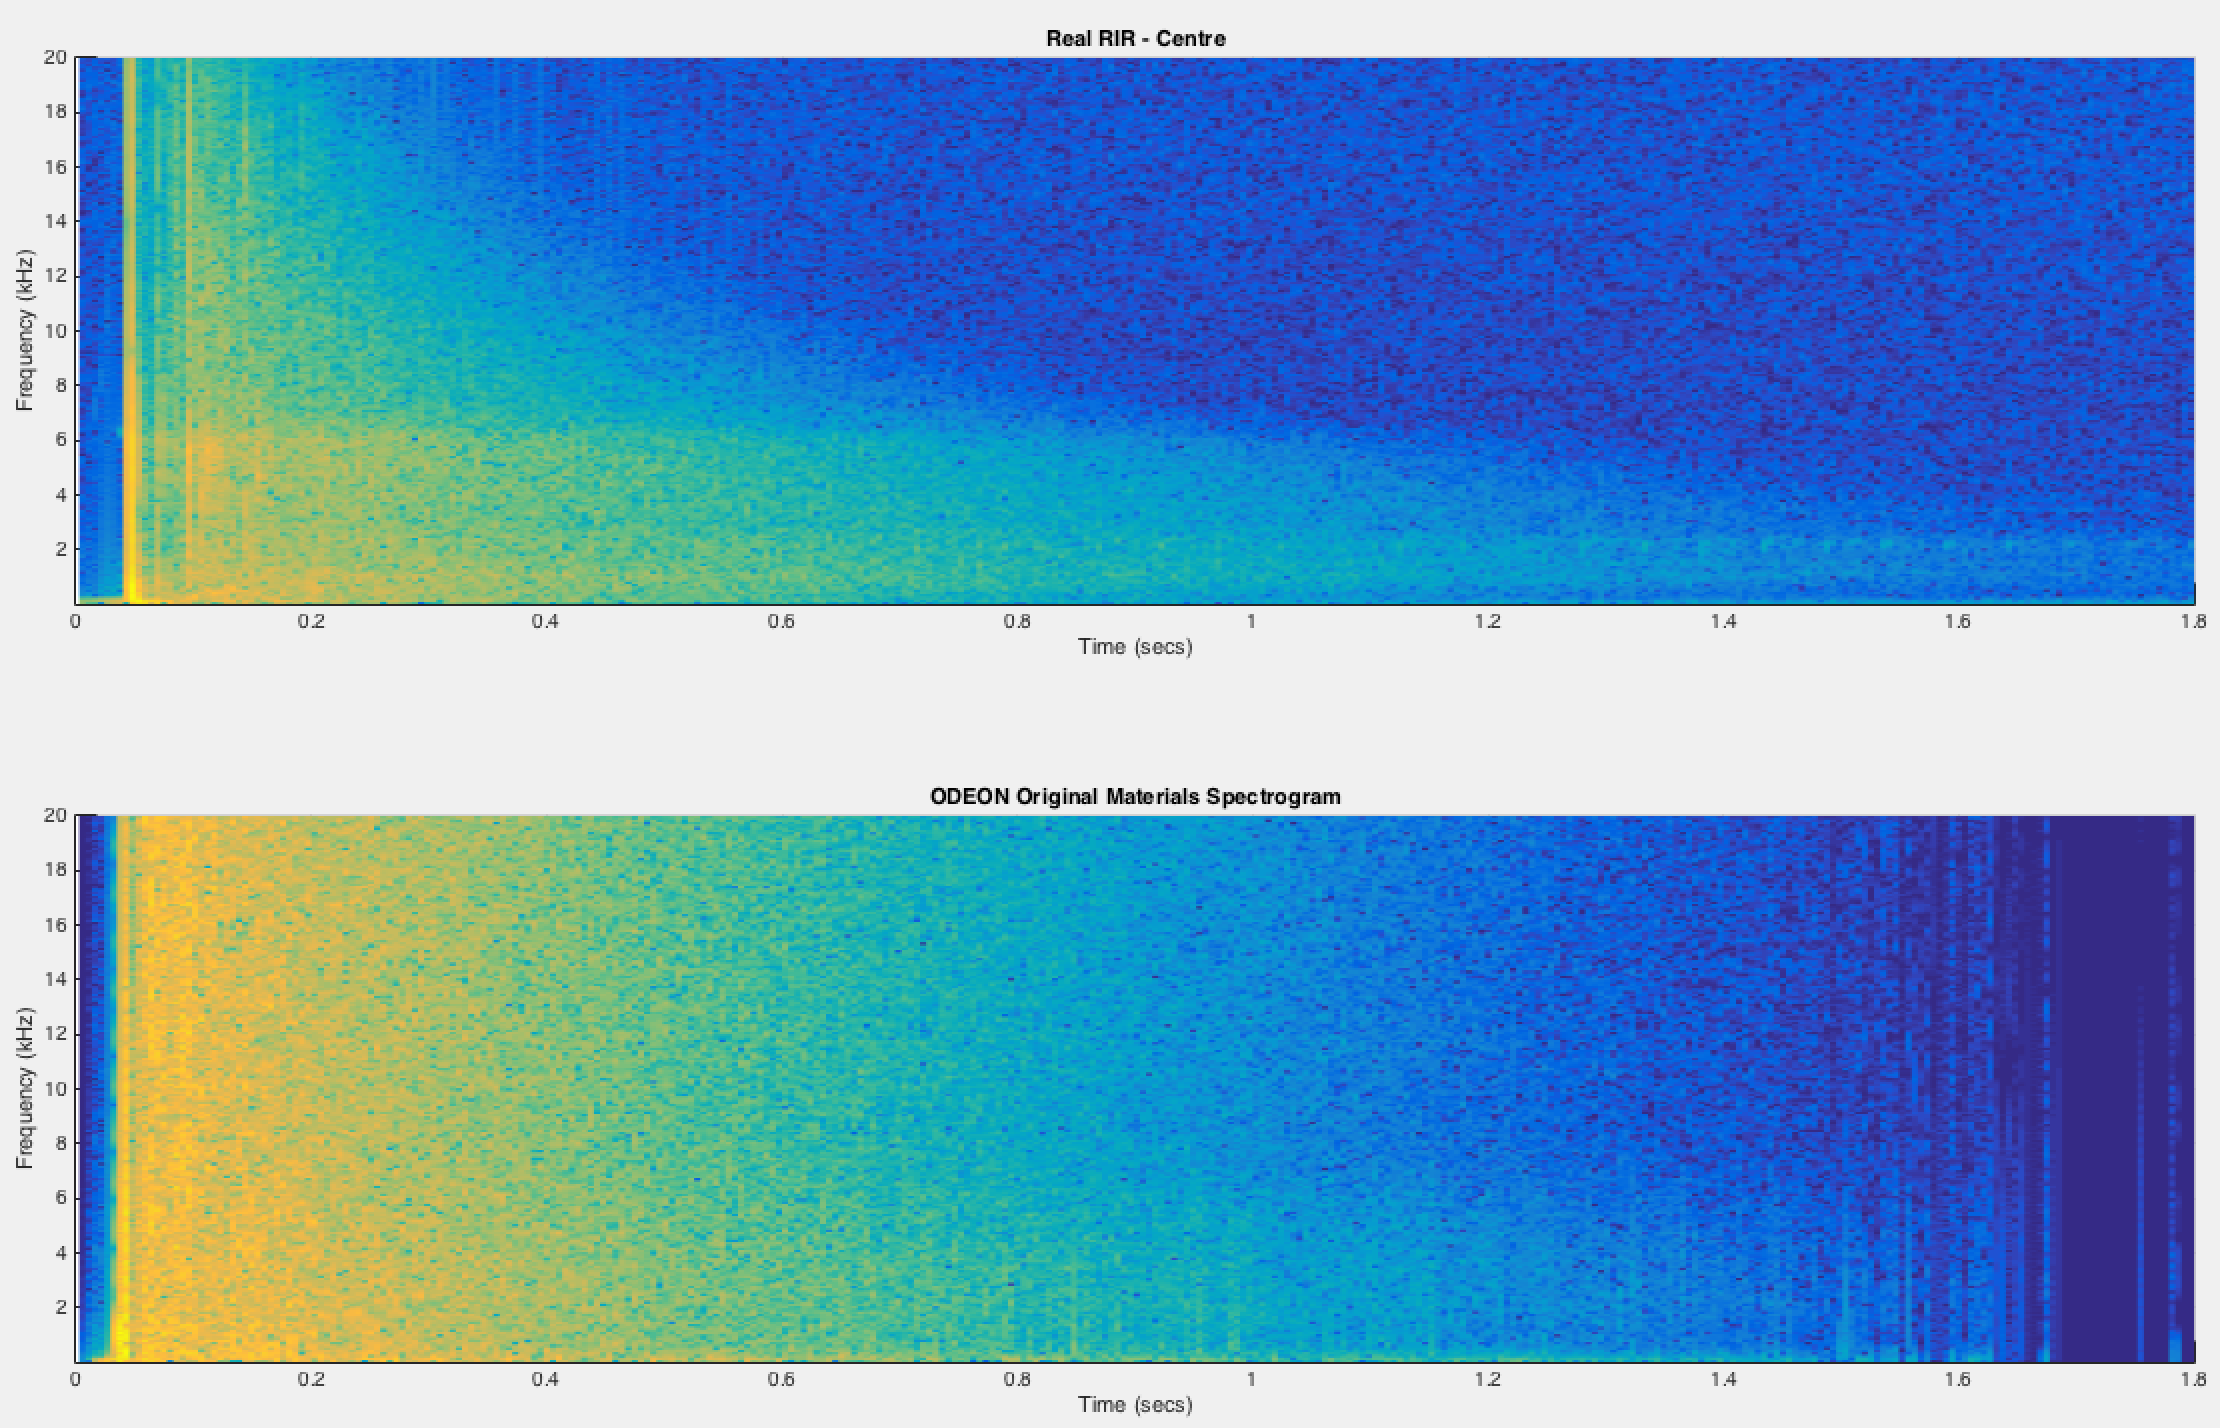
\includegraphics[scale = 0.3]{Sections/Implementation/Odeon/images/MaterialCompare/OriginalMaterials/original.png}
				\caption{Spectrograms of real \ac{RIR} (top) against spectrogram of first rendered \ac{RIR} from Odeon.}
				\label{compareOriginal}
			\end{figure}

			In an attempt to produce a more realistic synthetic \ac{RIR} the surface materials were edited several times until .

			 As the most obvious difference between the two is the difference in high frequency attenuation, large surfaces with low valued high frequency absorption coefficients such as the walls and ceiling were edited to absorb more of the high frequency content. Several iterations can be seen in figure~\ref{compareAll} showing the spectrogram of the real \ac{RIR} and several iterations of the \ac{RIR}'s rendered from Odeon. The Spectrogram at the bottom is that of an \ac{RIR} produced in Odeon with the final material selections. The difference between the real RIR and the final Odeon \ac{RIR} can be seen in figure~\ref{compareNew}. This was done by adding 10\% onto the existing absorption coefficients for the 63Hz - 2000Hz octave bands, 20\% to the 4000Hz band and 30\% to the 8000Hz band. This also included edited the ceiling material coefficients by adding an extra 10\% to the 8000Hz octave band.

			The following table contains a list of audio samples and edits made to the material list in order to produce each one, with their corresponding spectrogram graph name which can be found in figure~\ref{compareAll}.

			%-------------Audio Samples Table-------------%
			\begin{table}[H]
				\centering
				\begin{tabular}{|l | l | c | c | c |} 
					\hline
					\multirow{2}{*}{\textbf{Audio file}} & \multirow{2}{*}{\textbf{Graph Name}} & \multicolumn{3}{c|}{\textbf{Absorption Coefficient Edits}} \\ \cline{3-5}
					 & & \textbf{Material} & \textbf{Addition} & \textbf{Octave band} \\ \hline
					RealRIR.wav & Real RIR & \multicolumn{3}{c|}{NA}\\ \hline
					OdeonOriginal.wav & ODEON Original & \multicolumn{3}{c|}{NA}\\ \hline
					Odeon3RIR.wav & ODEON 3 & Ceiling (Mineral Fibre) & +10\% & 8kHz\\ \hline
					Odeon6RIR.wav & ODEON 6 & Walls (Solid Brick) & +10\% & All\\ \hline
					Odeon7RIR.wav & ODEON 7 & Walls (Solid Brick) & +10\% & 4kHz\\ 
					& & & +20\% & 8kHz \\
					& & Ceiling (Mineral Fibre) & +10\% & 8kHz\\ \hline
				\end{tabular}
				\caption{List of audio samples with corresponding spectrogram title in figure~\ref{compareAll} and the edits made for each one.}
				\label{materialTable}
			\end{table}

			%Material selection conclusion
			By analysing figure~\ref{compareNew} it can be seen that it was possible to produce a much more fitting \ac{RIR} compared to the one produced using the original materials. By listening to the audio samples, it is clear that though the final Odeon RIR (Odeon7RIR.wav) is much more similar to the real \ac{RIR} (RealRIR.wav) than the one produced using the original surface materials (OdeonOriginal.wav) in terms of reverberation time, they still sound very different in terms of their frequency content, where the \ac{RIR}'s produced in Odeon lack what the author considers \textit{depth}. This is most likely due to the fact that the geometrical acoustic modelling methods used to produce the \ac{RIR} do not accurately reproduce the low-frequency content, the reasons for which were discussed in section~\nameref{SoftwareOdon}

			\begin{center}
				\textbf{[Consider adding more detail of material selection process here]}
			\end{center}

			%-------------All materials compare-------------%
			\begin{figure}[H]
				\center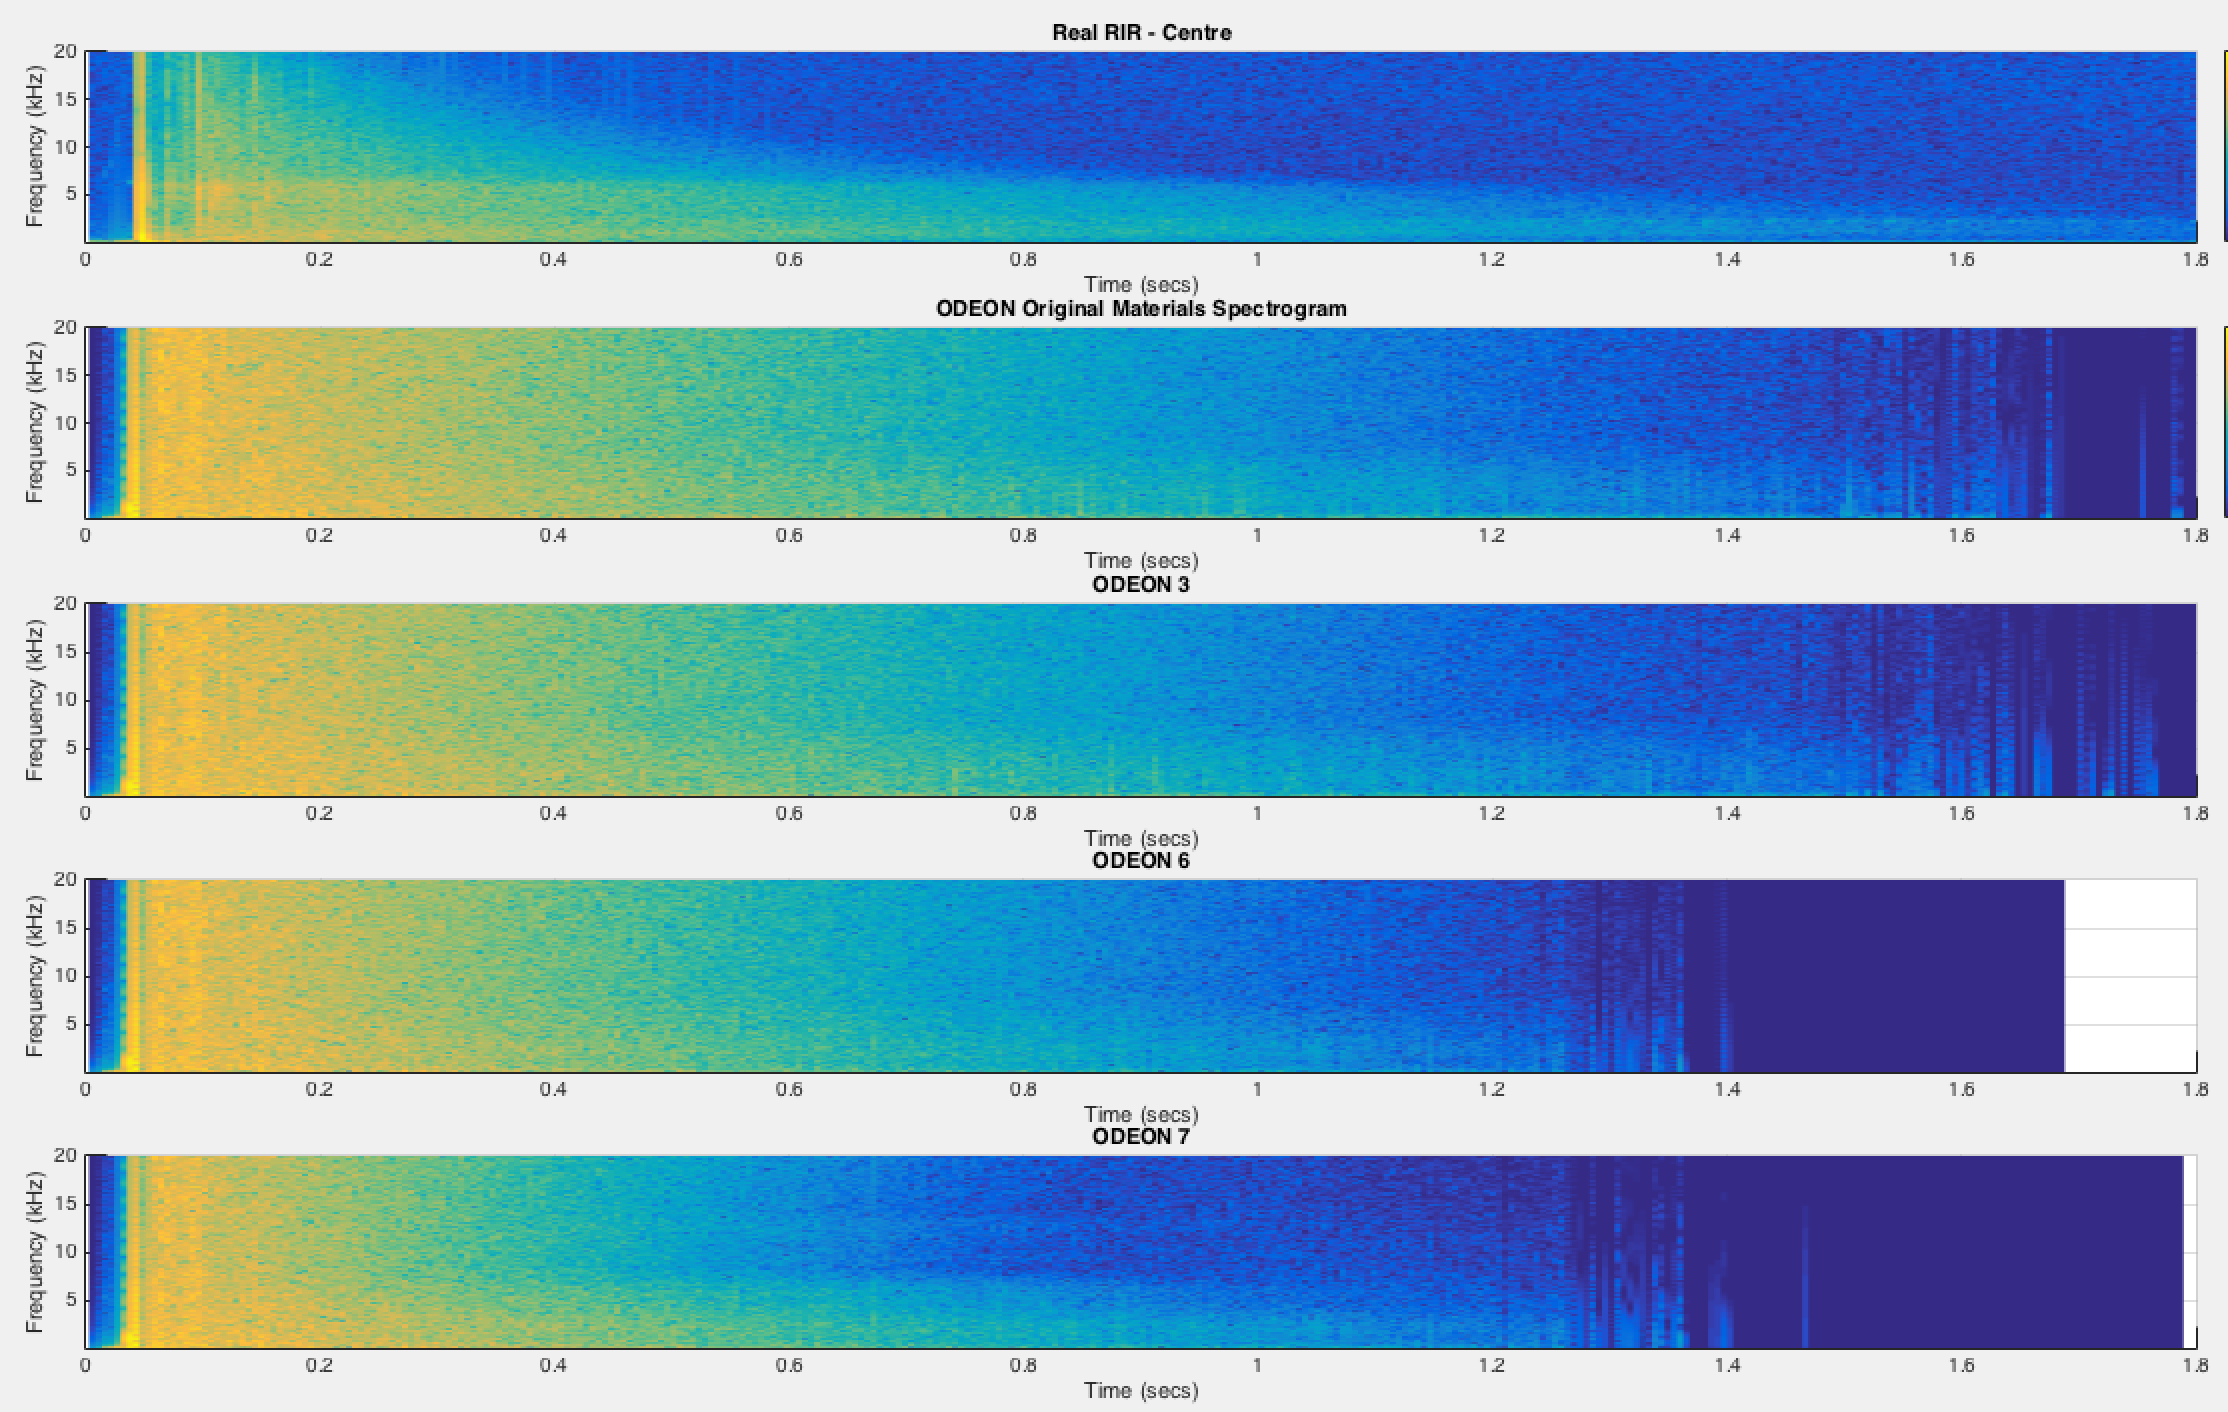
\includegraphics[scale = 0.4]{Sections/Implementation/Odeon/images/MaterialCompare/OriginalMaterials/all.png}
				\caption{Spectrograms of real \ac{RIR} (top) against spectrogram of several rendered \ac{RIR} from Odeon with different material absorption coefficients where ODEON  (bottom) shows the final \ac{RIR} used.}
				\label{compareAll}
			\end{figure}

			%-------------New materials compare-------------%
			\begin{figure}[H]
				\center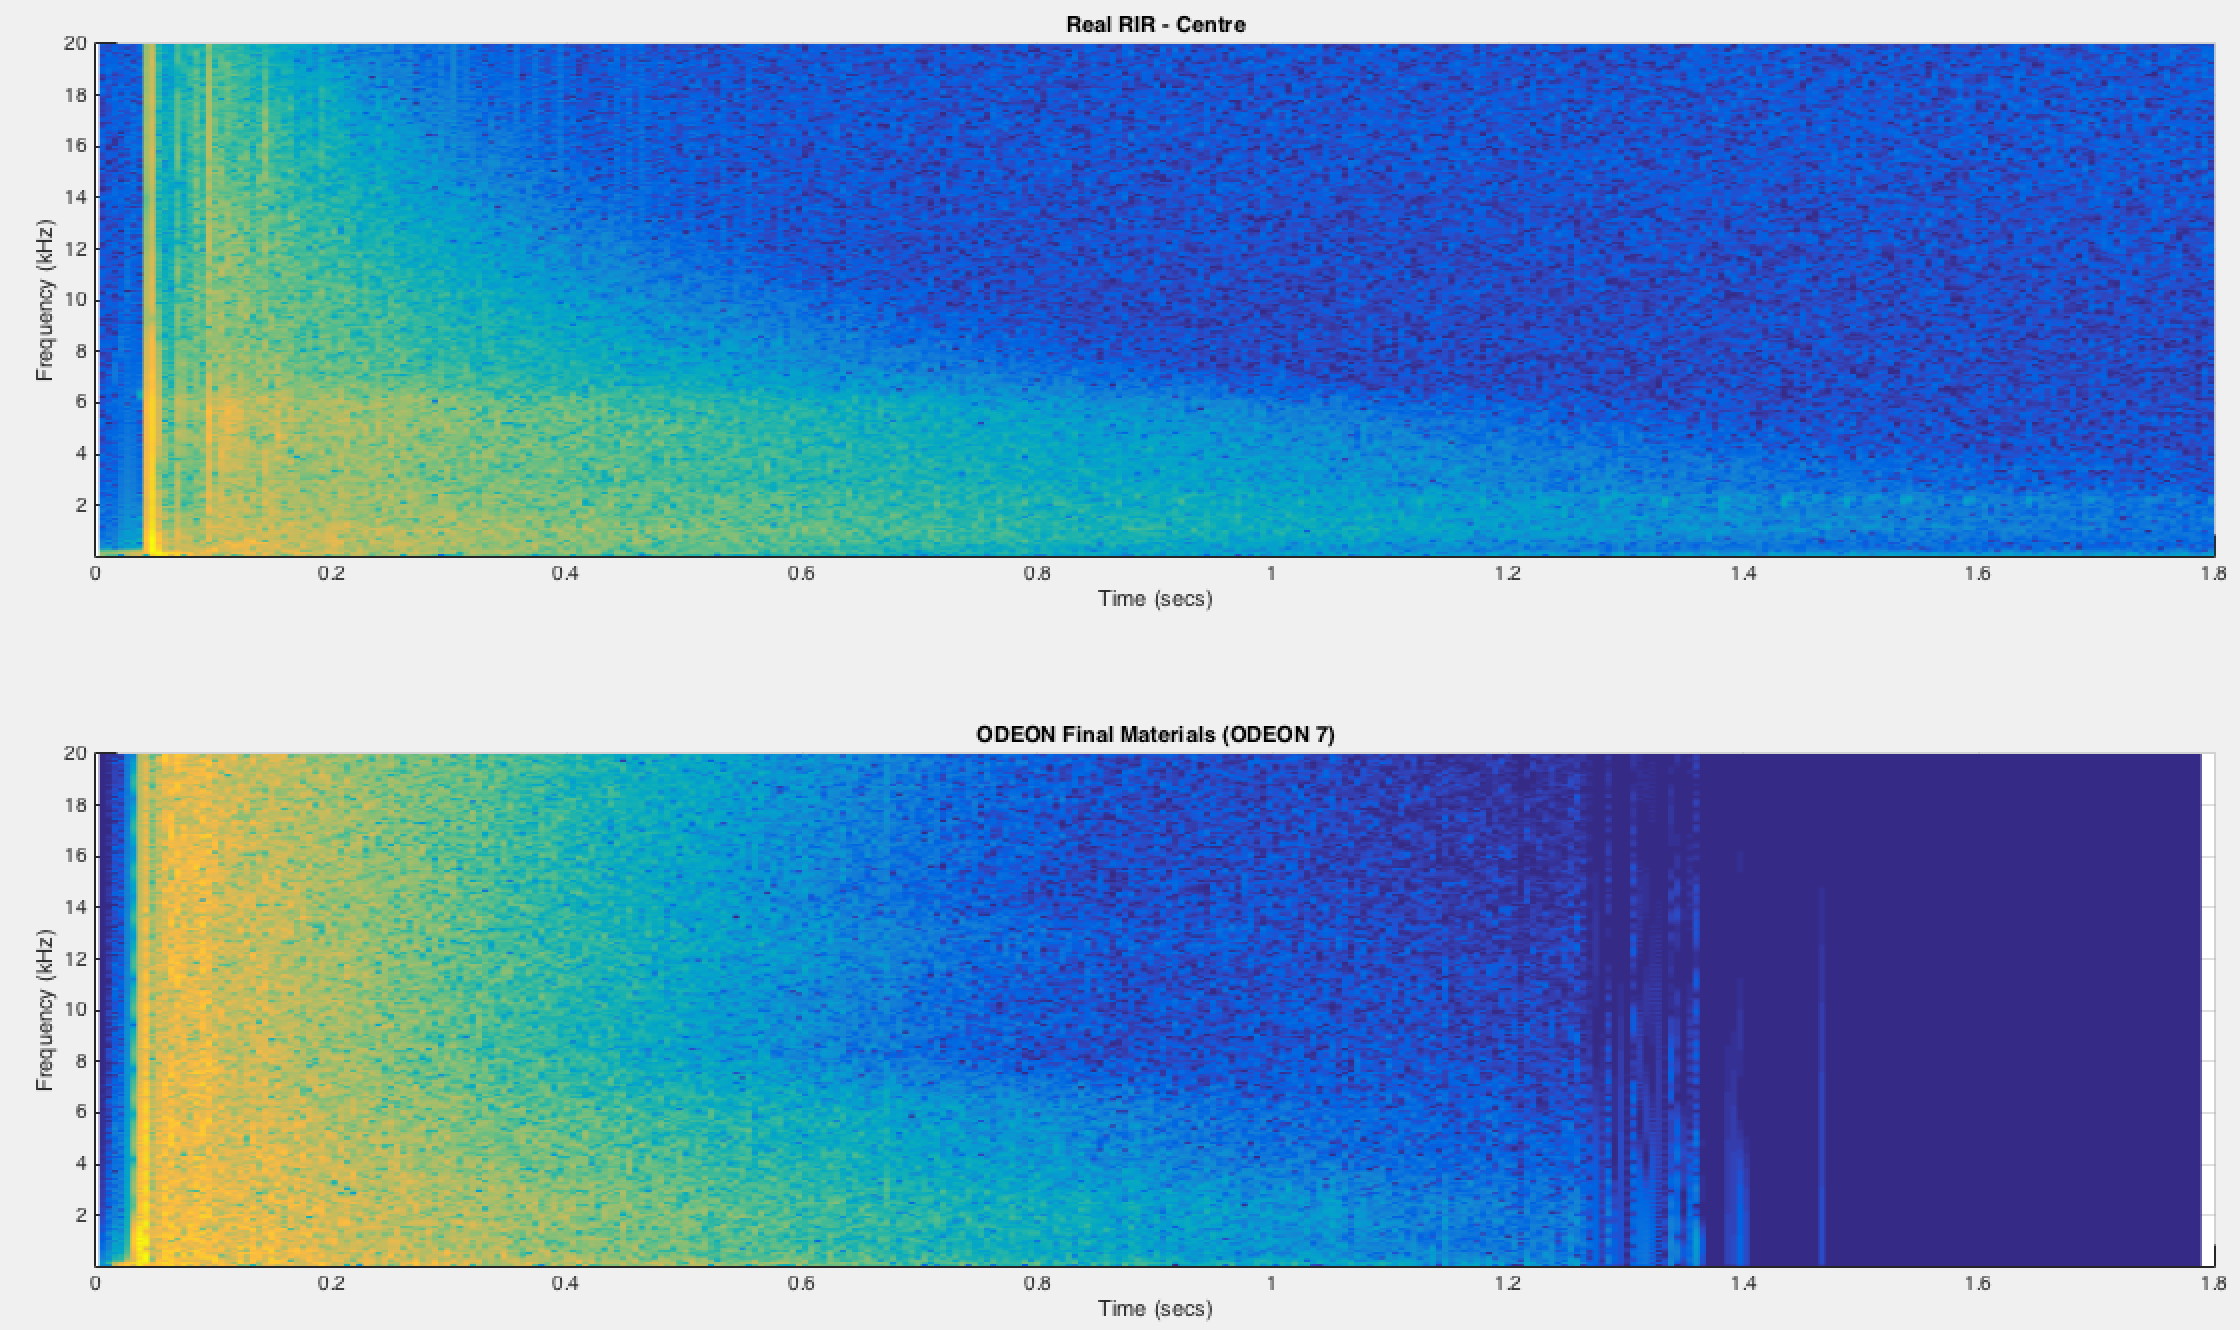
\includegraphics[scale = 0.3]{Sections/Implementation/Odeon/images/MaterialCompare/OriginalMaterials/new.png}
				\caption{Spectrograms of real \ac{RIR} (top) against Odeon \ac{RIR} from Odeon with final material absorption coefficients.}
				\label{compareNew}
			\end{figure}

			A full material list is available in `\texttt{Material\_List\_V2.xlsx}', showing which materials are applied to each surface within the Odeon model.

			%Mention incorrect RIRs
			It was later discovered (see section~\nameref{odeonError}) that the \ac{RIR}'s used to decide the final materials were incorrect, a result of which caused them to be much louder than they should have been. To ensure that the materials selected when using the incorrect \ac{RIR}'s were still appropriate for the new ones, two new \ac{RIR}'s were exported with the original materials and the final materials selected and plotted to compare against the same real \ac{RIR} used before. As the new Odeon \ac{RIR}'s were so much quieter, the real \ac{RIR} was reduced in level to match those produced by Odeon. The results are shown in figure~\ref{compareCorrect}. As it can be seen, the final materials used in the room model reduce the length of the reverb and attenuate high frequencies quicker than when the room model contained the original materials, the match is still not perfect.  

			%-------------Correct RIR materials compare-------------%
			\begin{figure}[H]
				\center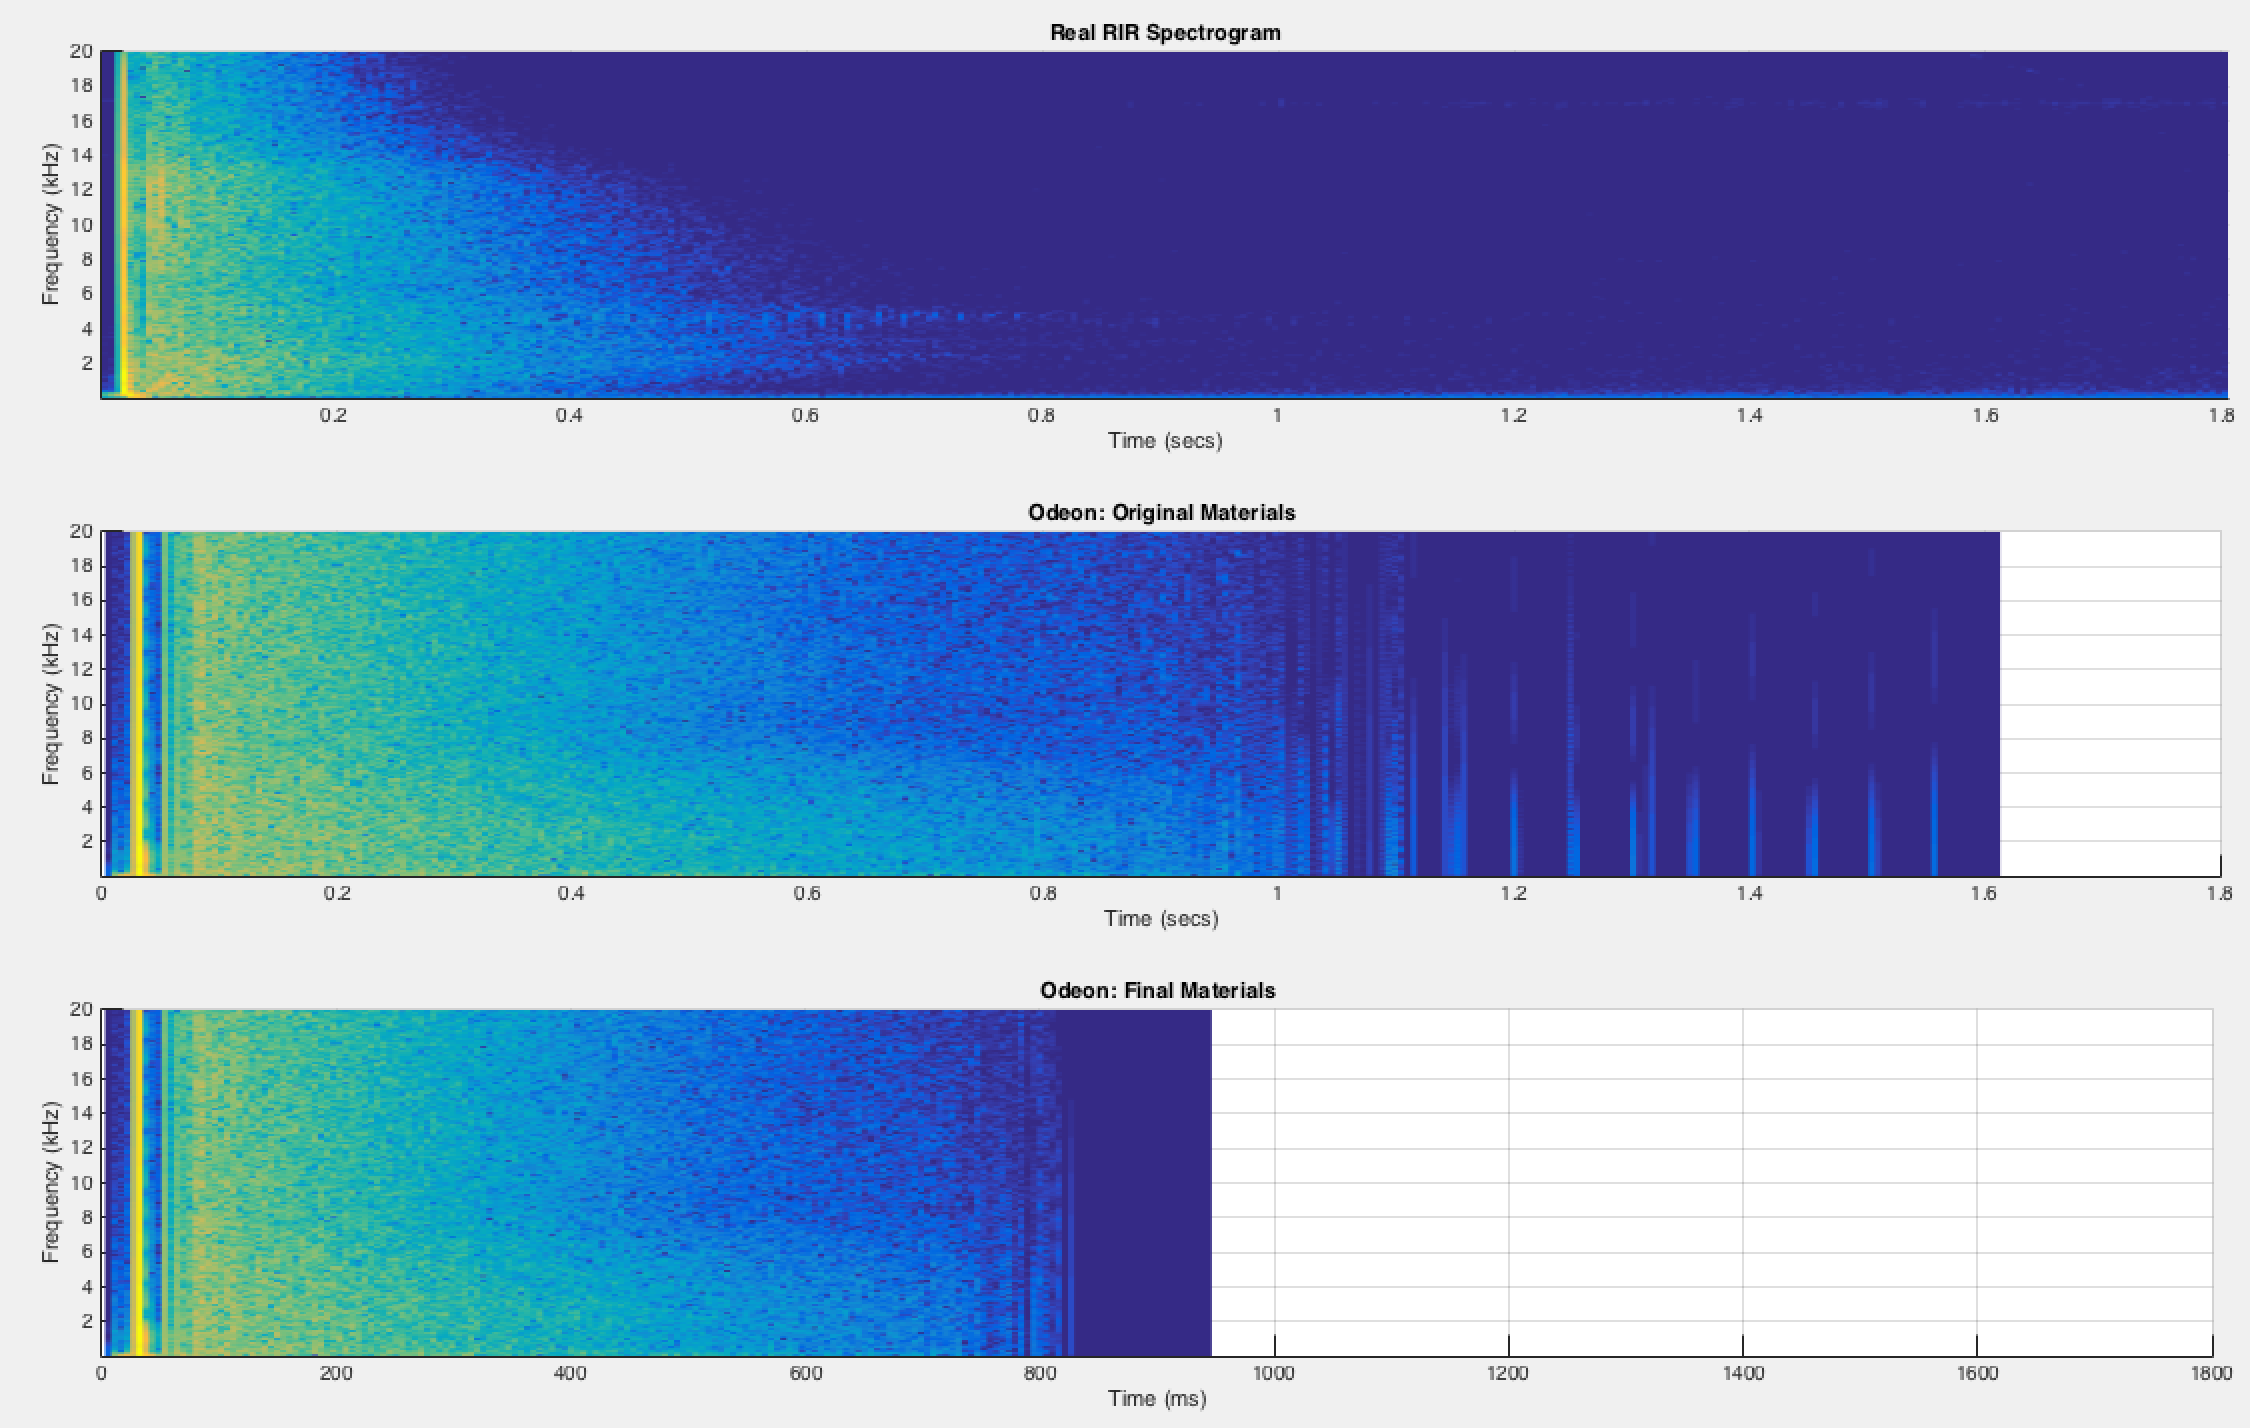
\includegraphics[scale = 0.4]{Sections/Implementation/Odeon/images/MaterialCompare/NewMaterials/newOdeonComparison.png}
				\caption{Spectrograms of correct Odeon \ac{RIR}'s with original materials (top) and final materials (center) to compare against real RIR that has been level calibrated (bottom).}
				\label{compareCorrect}
			\end{figure}

			\textbf{NOTE: The reason the Real RIR looks so different to the previous one is because it is much quieter, therefore the spectrogram shows less energy much earlier on. However the roll off described the first time is still present and is highlighted, starting again from about 0.2 seconds in. Why do the Odeon RIRs look similar to before then?}

			%RIR calibration for comparison

			%Show that new RIRs are okay


		\paragraph{Final Material Choice}

			

			The incorrect \ac{RIR}'s were used to calculate the room materials to begin with. Upon rendering new \ac{RIR}'s, three tests \ac{RIR}'s were rendered with the three main differences in materials selection in order to check that the spectrogram was close enough to the real \ac{RIR}'s

		\subsubsection{Odeon Output Settings}
			\paragraph{Ray Settings}

				%Other settings
				Odeon provides the following options for \ac{RIR} rendering:

				% \begin{center}
				% 	\begin{tabular}{p{3cm} | p{10cm}}
				% 		\textbf{Setting} & \textbf{Description (from~\cite{odeonManual})} \\ \hline
				% 		Astop (dB) & The maximum possible attenuation of each octave band. \\
				% 		Apass & Ripple of octave band filters in dB\\
				% 		Band overlap & 100\% overlap gives a smooth transition between the FIR octave band filters as they are not completely rectangular \\
				% 		Maximum reflection order & Maximum allowed is 2000 as is the default. This means a ray can only reflect around a room 2000 times before the simulation is stopped. This prevents trapped rays from prolonging the impulse response if it never reaches the receiver. \\
				% 		Late Rays & These are emitted from the source and reflected according to the \ac{VBS} (described in section~\nameref{background:scattering}) taking into account scattering due to surface size and roughness. If the reflection order is about the transition order, a secondary source is generated at each reflection point.\\
				% 		Transition Order & As explained in section~\nameref{Software:Odeon}, a \ac{TO} can be set to determine the number of early rays sent out to find a number of wall combinations for reflections using the \ac{ISM}. After this number of rays has been reached, the ray-tracing method is used.
				% 	\end{tabular}
				% \end{center}

				\textbf{Astop} - The maximum possible attenuation of each octave band.
				\textbf{Apass} - Ripple of octave band filters in dB.

				\textbf{Band overlap} - 100\% overlap gives a smooth transition between the FIR octave band filters as they are not completely rectangular.

				\textbf{Maximum reflection order} - Maximum allowed is 2000 as is the default. This means a ray can only reflect around a room 2000 times before the simulation is stopped. This prevents trapped rays from prolonging the impulse response if it never reaches the receiver.

				\textbf{Late Rays} - These are emitted from the source and reflected according to the \ac{VBS} (described in section~\nameref{background:scattering}) taking into account scattering due to surface size and roughness.

				\textbf{Transition Order} - As explained in section~\nameref{Software:Odeon}, a \ac{TO} can be set to determine the number of early rays sent out to find a number of wall combinations for reflections using the \ac{ISM}. After this number of rays has been reached, the ray-tracing method is used.


				All settings apart from \ac{LR's} and \ac{TO} are left at their default values as they are sufficient for accuracy and prevent the increase of computation time which will be needed given the large number of RIRs required for free movement.

				%TO and Late rays

				Odeon suggests two possible modes, \textbf{Engineer} and \textbf{Precision} which both suggest using a different number of \ac{LR's} which are 1285 and 20560 respectively. As both the \ac{TO} and \ac{LR's} value increase both the accuracy and computation time of the \ac{RIR}'s, these values were tried with difference combinations of \ac{TO} values and \ac{RIR}'s were rendered. Figure~\ref{odeonSettingsRIR} shows plots of the rendered \ac{RIR}'s with the name indicating the \ac{TO} and \ac{LR's} value. For example, `TO\_2\_LR\_1285' indicates the sample was produced where \ac{TO} = 2 and \ac{LR's} = 1285. Table~\ref{odeonSettingsTable} can be used to clarify the settings used for each \ac{RIR} in figure~\ref{odeonSettingsRIR} and indicates which audio sample can be listened to. All \ac{RIR}'s were taken from the centre of the room.

				\begin{table}
				\begin{center}
					\begin{tabular}{|l | c | l | l|}
					\hline
					\textbf{Audio Sample} & \textbf{\ac{TO}} & \textbf{\ac{LR's}} & \textbf{Graph Name}\\ \hline
					TO\_2\_LR\_1285.wav & 2 & 1285 & TO\_2\_LR\_1285 \\
					TO\_2\_LR\_20560.wav & 2 & 20560 & TO\_2\_LR\_20560 \\
					TO\_4\_LR\_1285.wav & 4 & 1285 & TO\_4\_LR\_1285\\
					TO\_4\_LR\_20560.wav & 4 & 20560 & TO\_4\_LR\_20560 \\ \hline
					\end{tabular}
				\end{center}
				\caption{Table of audio samples with the corresponding settings information and graph name}
				\label{odeonSettingsTable}
				\end{table}


			%-------------TO and LR value image-------------%
			\begin{figure}[H]
				\center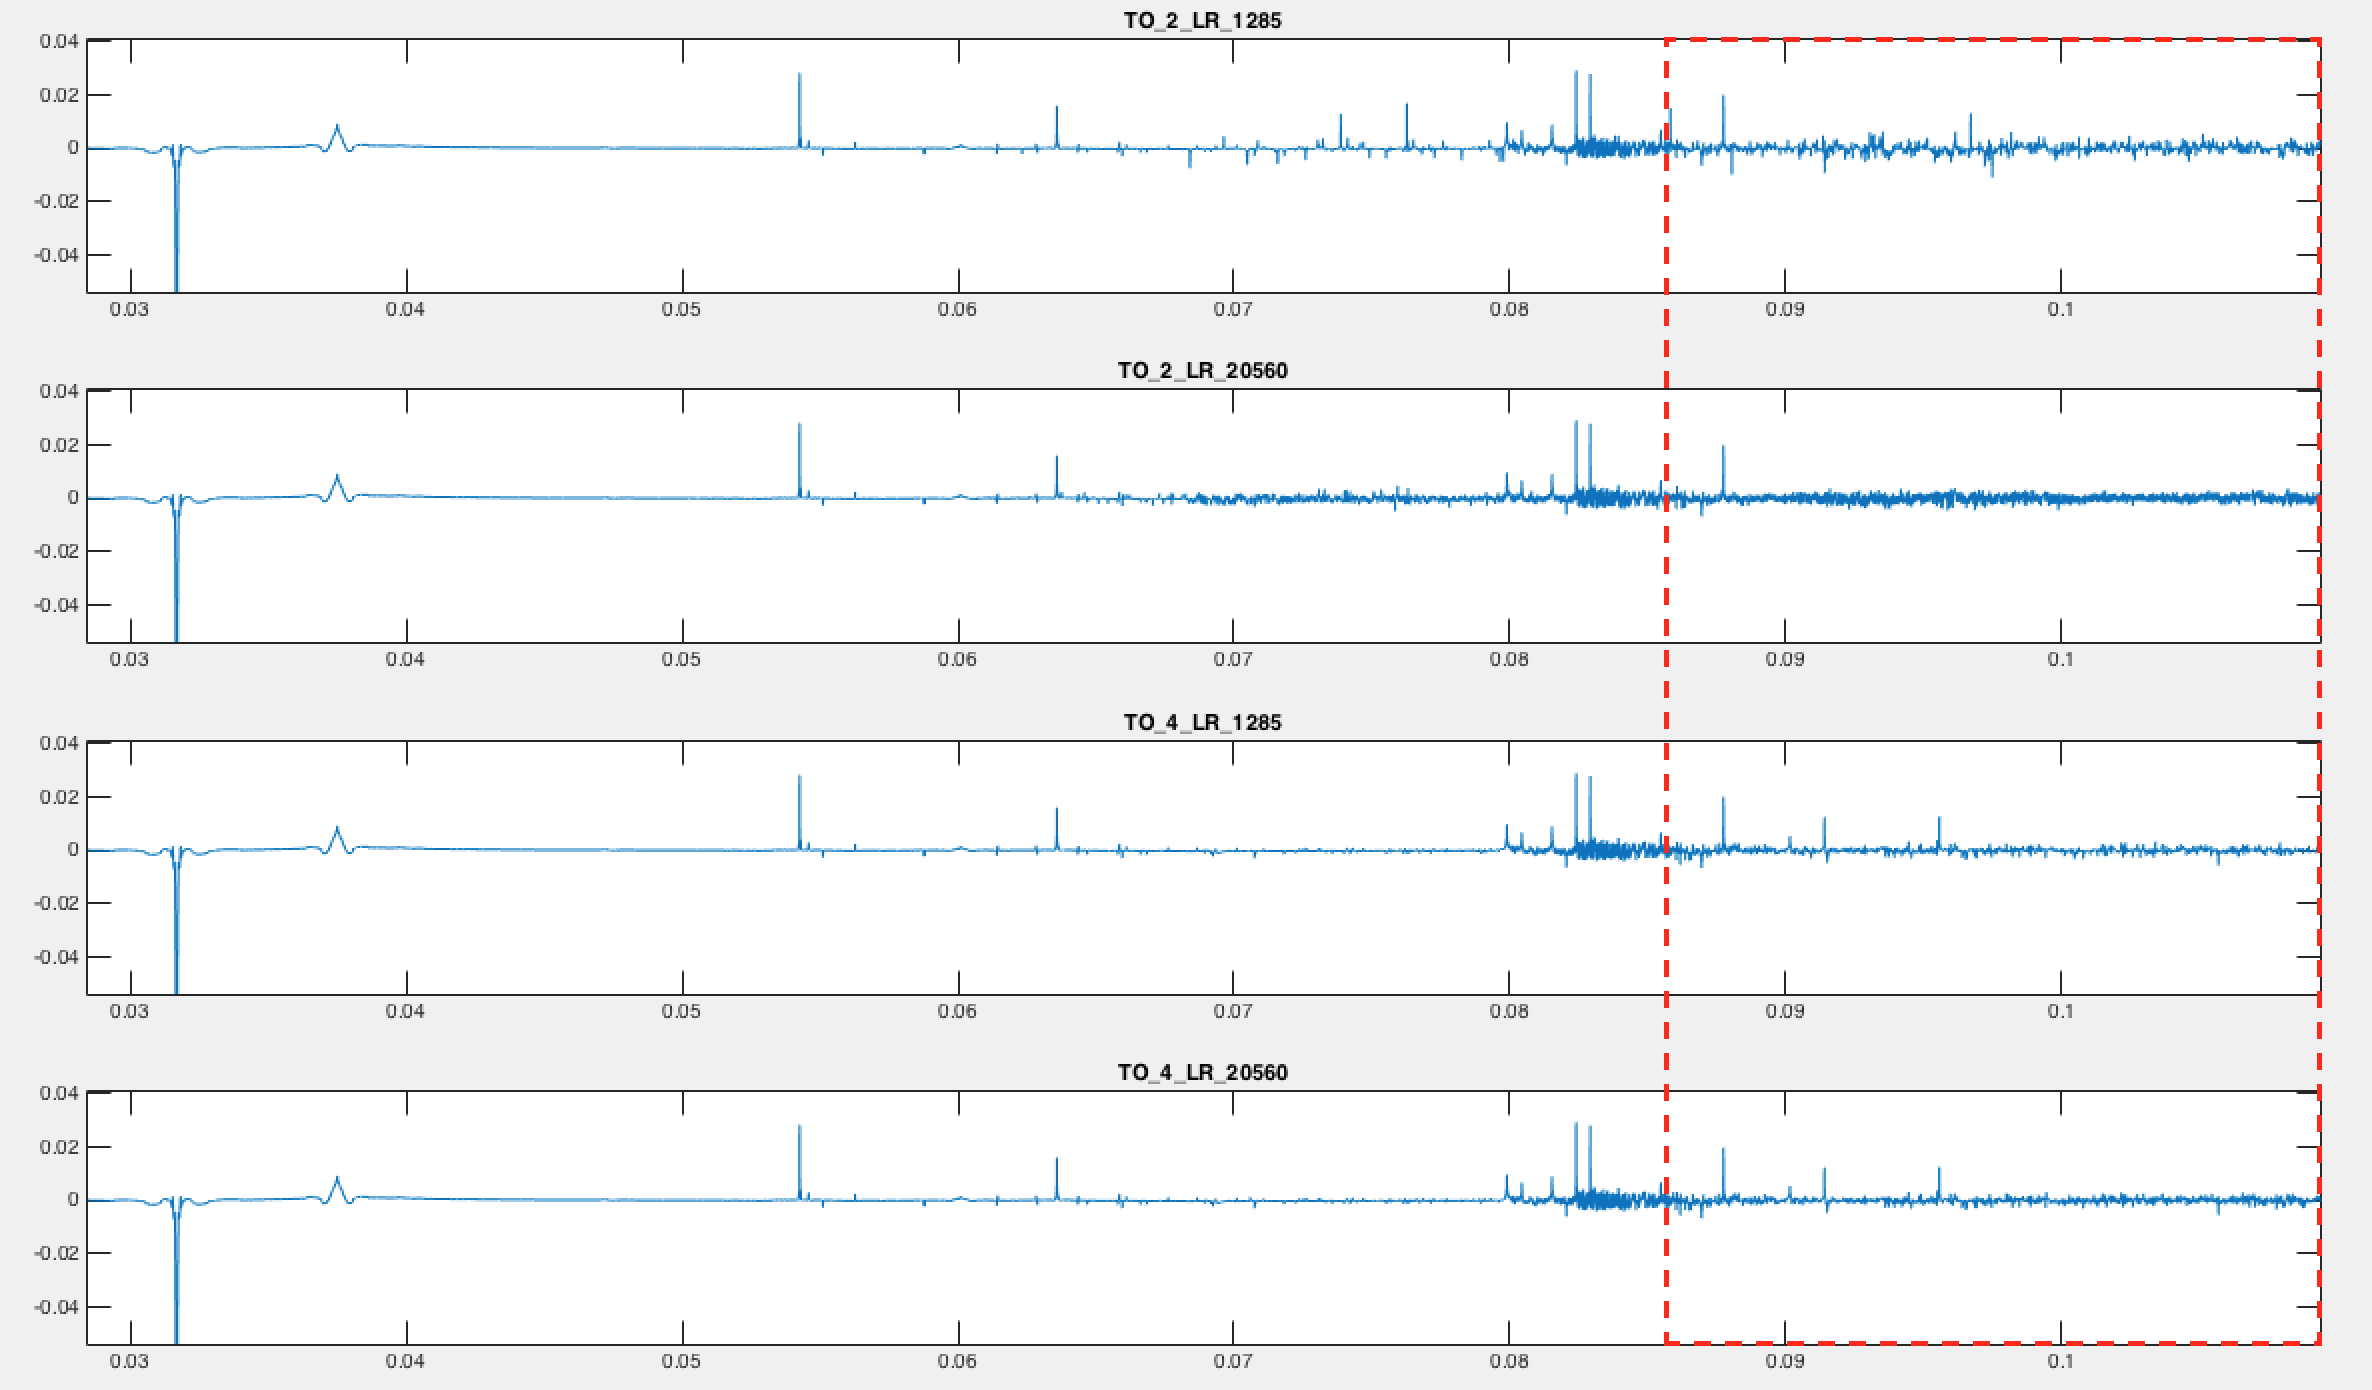
\includegraphics[scale = 0.4]{Sections/Implementation/Odeon/images/OdeonSettings/settingsFigure_edit.png}
				\caption{\ac{RIR}'s rendered using different \ac{TO} and late ray values}
				\label{odeonSettingsRIR}
			\end{figure}
				%-------------TO and LR value Zoomed image-------------%
			\begin{figure}[H]
				\center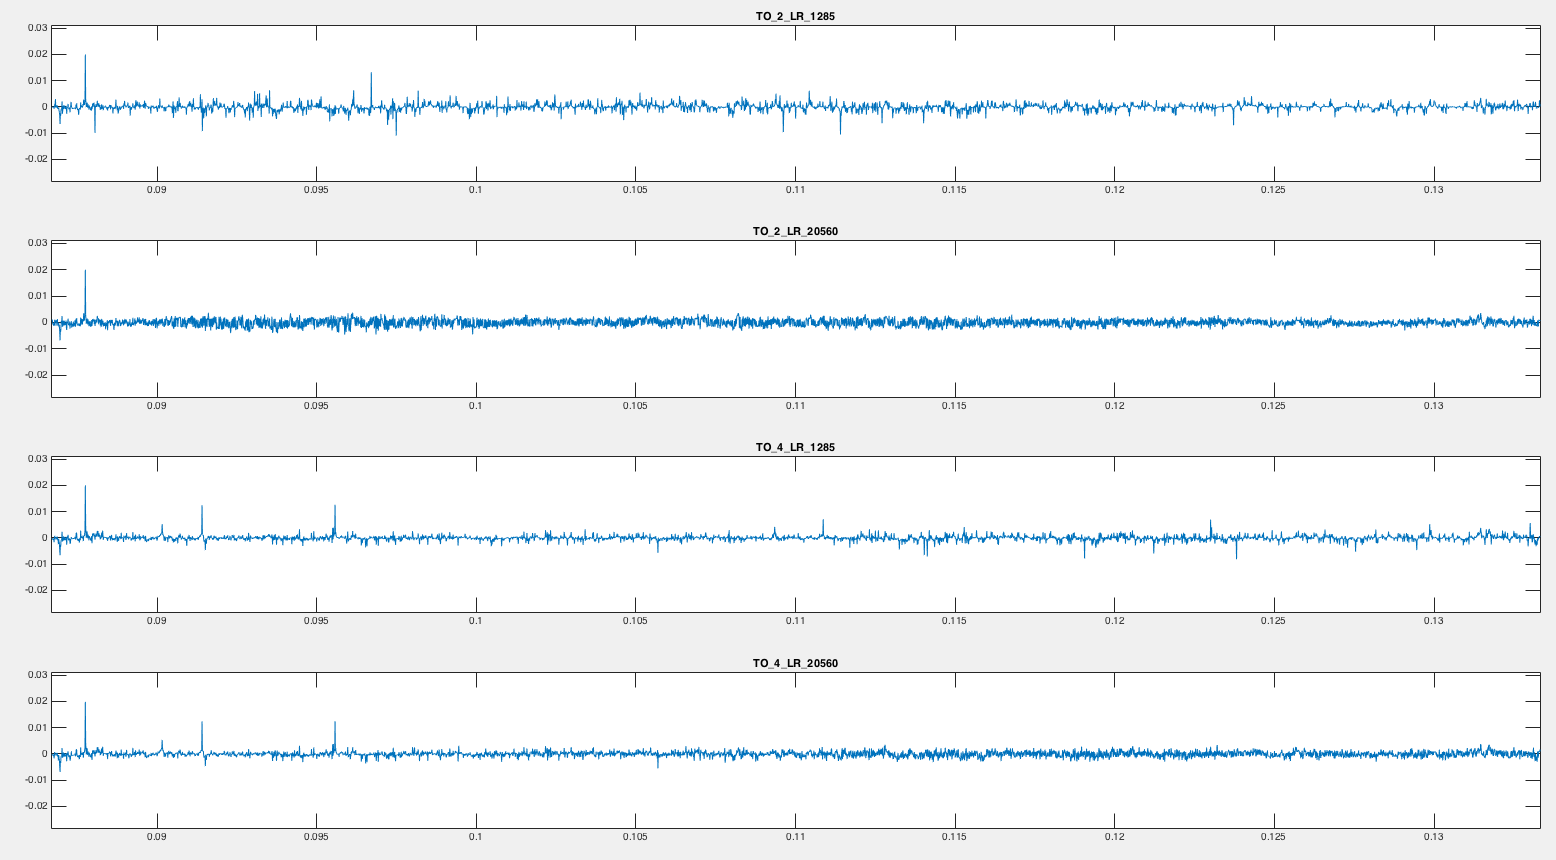
\includegraphics[scale = 0.3]{Sections/Implementation/Odeon/images/OdeonSettings/settingsFigureZoomed.png}
				\caption{Zoomed in section indicated by the red dashed line in figure~\ref{odeonSettingsRIR}}
				\label{odeonSettingsRIRZoomed}
			\end{figure}

				%-------------TO Zoomed image-------------%
			\begin{figure}[H]
				\center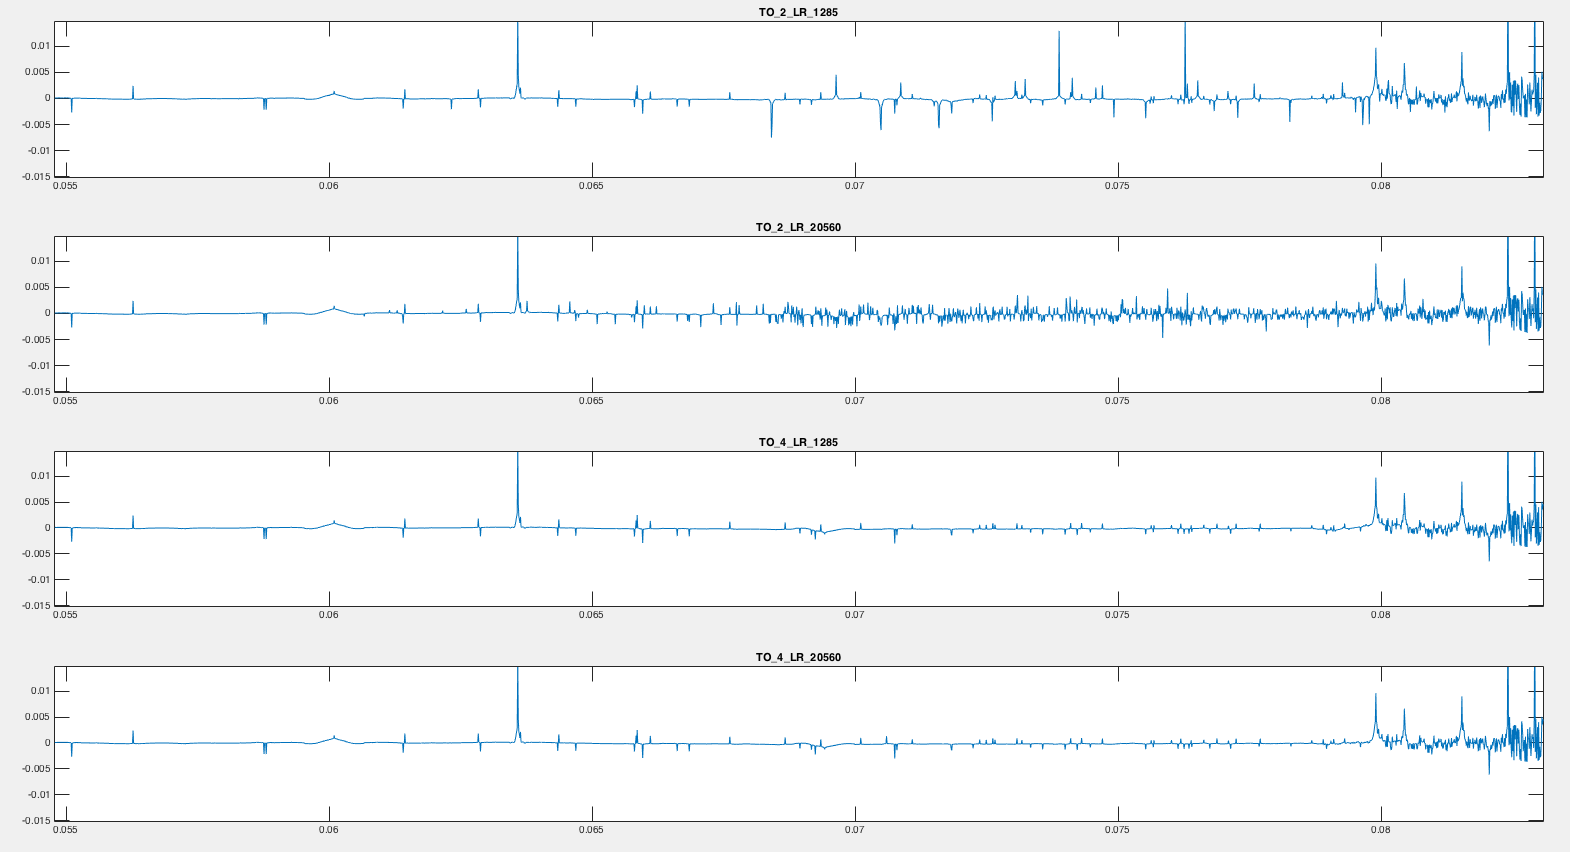
\includegraphics[scale = 0.3]{Sections/Implementation/Odeon/images/OdeonSettings/settingsFigure_TOZoom.png}
				\caption{Zoomed in section showing the effects of using a high \ac{TO} value}
				\label{odeonSettings_TOZoomed}
			\end{figure}


				\textbf{Audio samples: SupportingFiles/Audio/Odeon\_Settings}

				Through aural analysis, it can be heard that the number of \ac{LR's} used has an audible impact, where a lower \ac{LR's} value produces an \ac{RIR} that sounds more \textit{grainy}. This can be seen in figure~\ref{odeonSettingsRIRZoomed}, showing the \ac{RIR}'s in figure~\ref{odeonSettingsRIR} which have been zoomed to show the \ac{RIR} from approximately 0.085s where a difference caused by the different setting combinations can be seen. The two \ac{RIR}'s with a high \ac{LR's} value (2nd and 4th plot) show more densely packed reflections due to the fact that more rays are used. This produces a `smoother' more natural sounding reverb tail.

				Figure~\ref{odeonSettings_TOZoomed} shows an earlier part of the \ac{RIR}'s where the effect of using a high \ac{TO} value can be seen. The two plots showing the \ac{RIR}'s with a \ac{TO} of 2 show more random reflections earlier on where the ray-tracing method has been used, whereas the bottom two plots with a \ac{TO} of 4 show less random reflections as the \ac{ISM} will still be used. Though the difference in using a \ac{TO} of 2 or 4 can be seen, is not audible.

				The time difference taken to render the \ac{RIR}'s is also an important factor when choosing which of these settings to use. Given the potentially large number of \ac{RIR}'s required, a slightly more accurate output may result in a much greater calculation time. Odeon uses information gathered when previously rendering \ac{RIR}'s to speed up calculations for other \ac{RIR}'s being rendered in the same room, however there initial time taken to calculate each of the \ac{RIR}'s was noted and compared for reference.

				Initially it was found that increasing the \ac{TO} from 2 to 4 increased the time taken to render by approximately 20 seconds. However, It was later realised that inaccurate calulation times may have been given due to the fact the project was being stored on the University network, thus adding variable delay times. The project was later stored on a local C drive, eliminating any network speed issues and inconsistencies. After doing so, the difference in \ac{TO} values made almost no difference to the calculation times. In hindsight, a higher \ac{TO} value could have been used to produce more accurate \ac{RIR}'s.

				It was found that the \ac{LR's} value made quite a difference to the calculation time:

				\begin{center}
					\begin{tabular}{c l c}
					\textbf{Transition Order} & \textbf{Late Ray Value} & \textbf{Calculation Time (s)} \\ \hline
					2 & 1285 & 11 \\
					2 & 20560 & 28 \\
					4 & 1285 & 11 \\
					4 & 20560 & 28 \\
					\end{tabular}
				\end{center}

				Despite the increase in calculation time by 17 seconds, the inaccuracy of \ac{RIR}'s produced when using the lower \ac{LR's} makes using the higher value justifiable.

				%B-Format setting
				As the \ac{VSS} requires B-format audio files, the B-format option was selected.



			\paragraph{Directivity}

				%Possible to use CLF2 to mimic sound source directivity
				Without selecting otherwise, Odeon uses an omni-directional point source as the sound source. This can be changed however by providing a .cf2 file. This file stores loudspeaker performance data and polar plots in what is known as a Common Loudspeaker Format, a standard used by loudspeaker manufacturers. By importing one of these files, Odeon simulates the directionality of the selected loudspeaker as the sound source. This can be used to attempt to more accurately recreate an \ac{RIR} that would be taken in a real space, by finding the .cf2 file that corresponds to the loudspeaker used for the measurement.

				It is also possible however, to input a custom directivity pattern to model a specific sound source. This provides an opportunity to create a more accurate sound source for a human head, something desirable when creating \ac{RIR}'s that will be convolved with the audio input from a singer. Techniques for recording the directivity of the human head have been reviewed and improved upon in \cite{Monson2012b}, however only directivity data for the horizontal plane was recorded. A student from the University of York has recently investigated the directivity of a human head in both the vertical and horizontal planes ranging from the 63Hz to 8kHz octave band \cite{calum} \textbf{[CHANGE NAME]} and generously provided said data to be used in this project. Figure~\ref{directivity} shows the directivity patten editor window in Odeon with the input horizontal and vertical directivity patterns for the 8Khz octave band taken from \cite{calum}. 


				%-------------Directivity Image image-------------%
				\begin{figure}[H]
					\center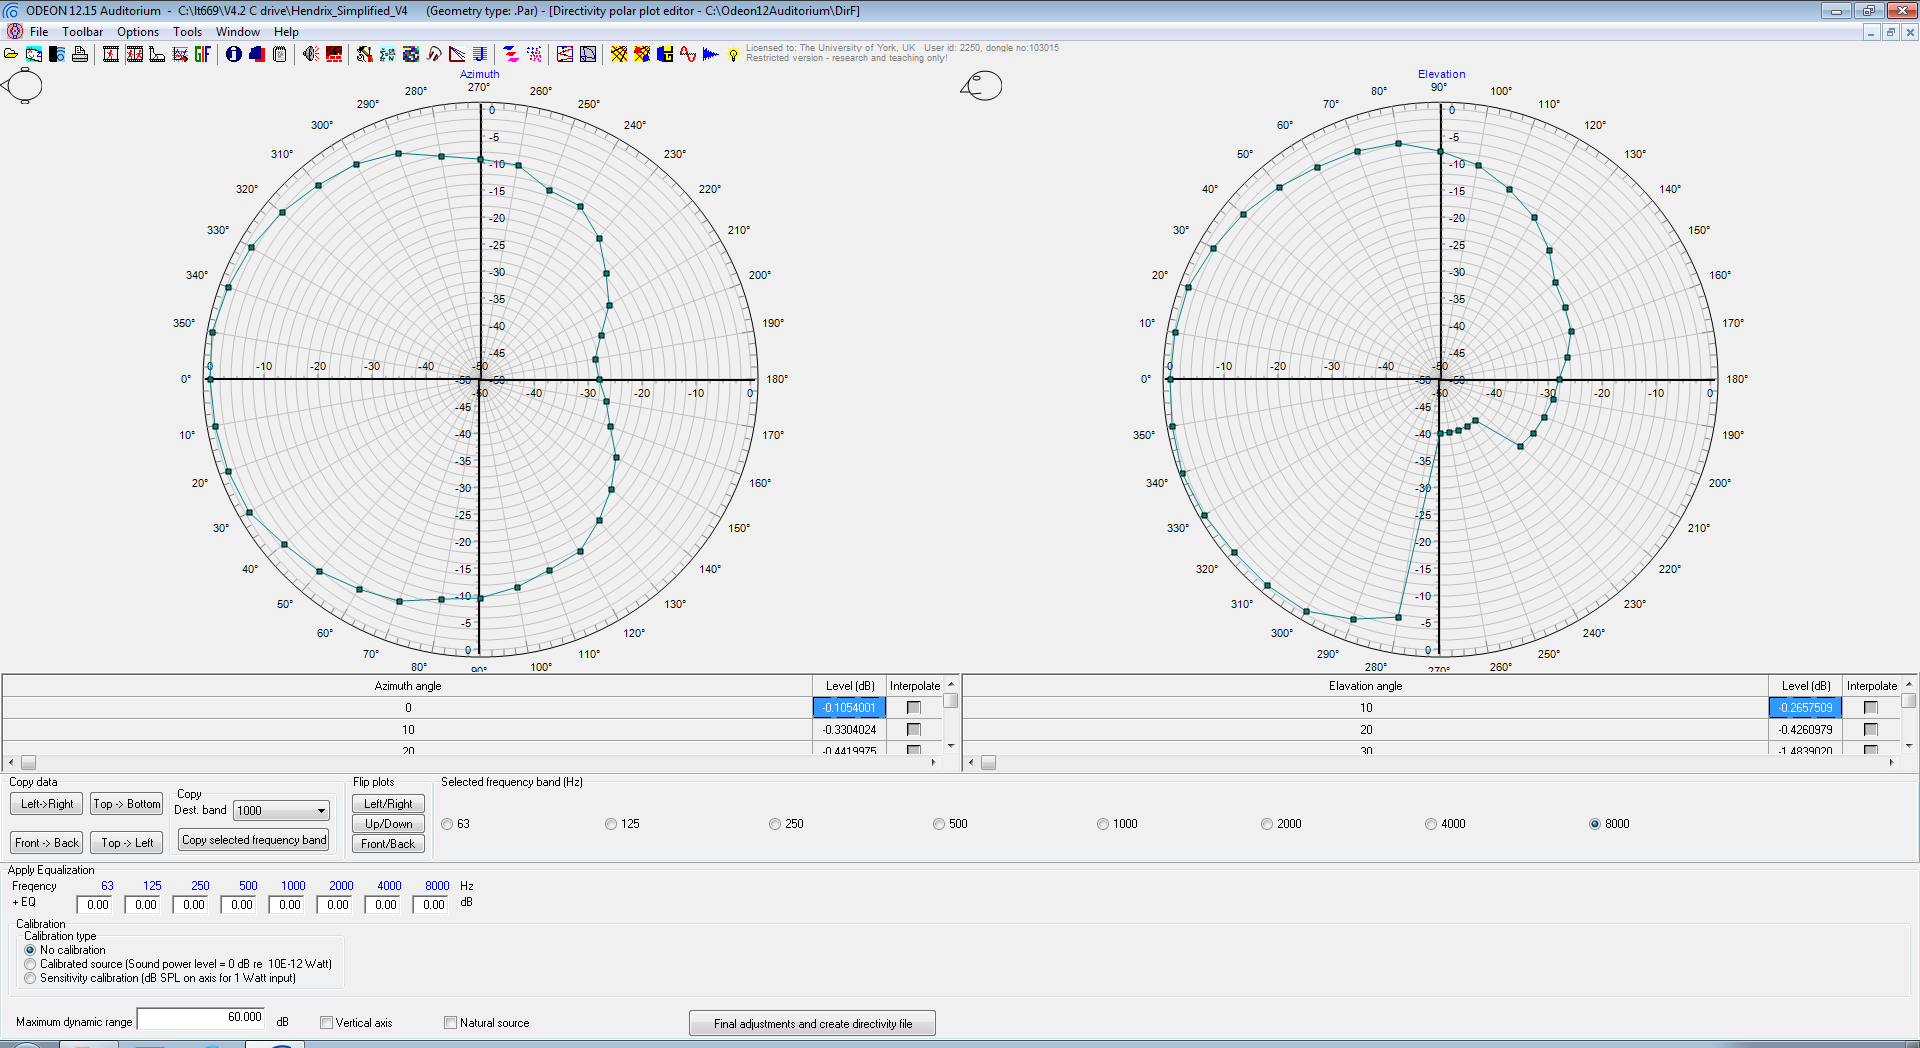
\includegraphics[scale = 0.3]{Sections/Implementation/Odeon/images/Directivity/DirectivityPattern.png}
					\caption{Directivity pattern editor window in Odeon showing the directivity pattern for the horizontal plane (left) and the vertical plane (right) for the 8Khz octave band using data from \cite{calum}}
					\label{directivity}
				\end{figure}


		\subsubsection{RIR Topology Problems}
		\label{odeonError}
			%Show original output RIR
			It has been noted that the \ac{RIR}'s produced will attempt to accurately resemble a human head. This involves placing the sound source below the receiver, to resemble the mouth (sound source) below the ears (receiver). When taking real \ac{RIR} measurements it is often not possible to get the source and receiver close enough due to the physical dimensions of the equipment used and therefore result in an unnatural distance between them (see section~\nameref{realRIRs}). However, with using software such as Odeon, where sound sources are calculated from a point source, it is possible to move the source and receiver much closer together. Initially, the sound source was place 1m off the ground and the receiver was positioned 0.05m above the sound source. Three \ac{RIR}'s positioned along the centre of the room at varying distances from the left wall can be seen in figure~\ref{incorrectRIR}.

			%Show timing errors


			%-------------Directivity Image image-------------%
			\begin{figure}[H]
				\center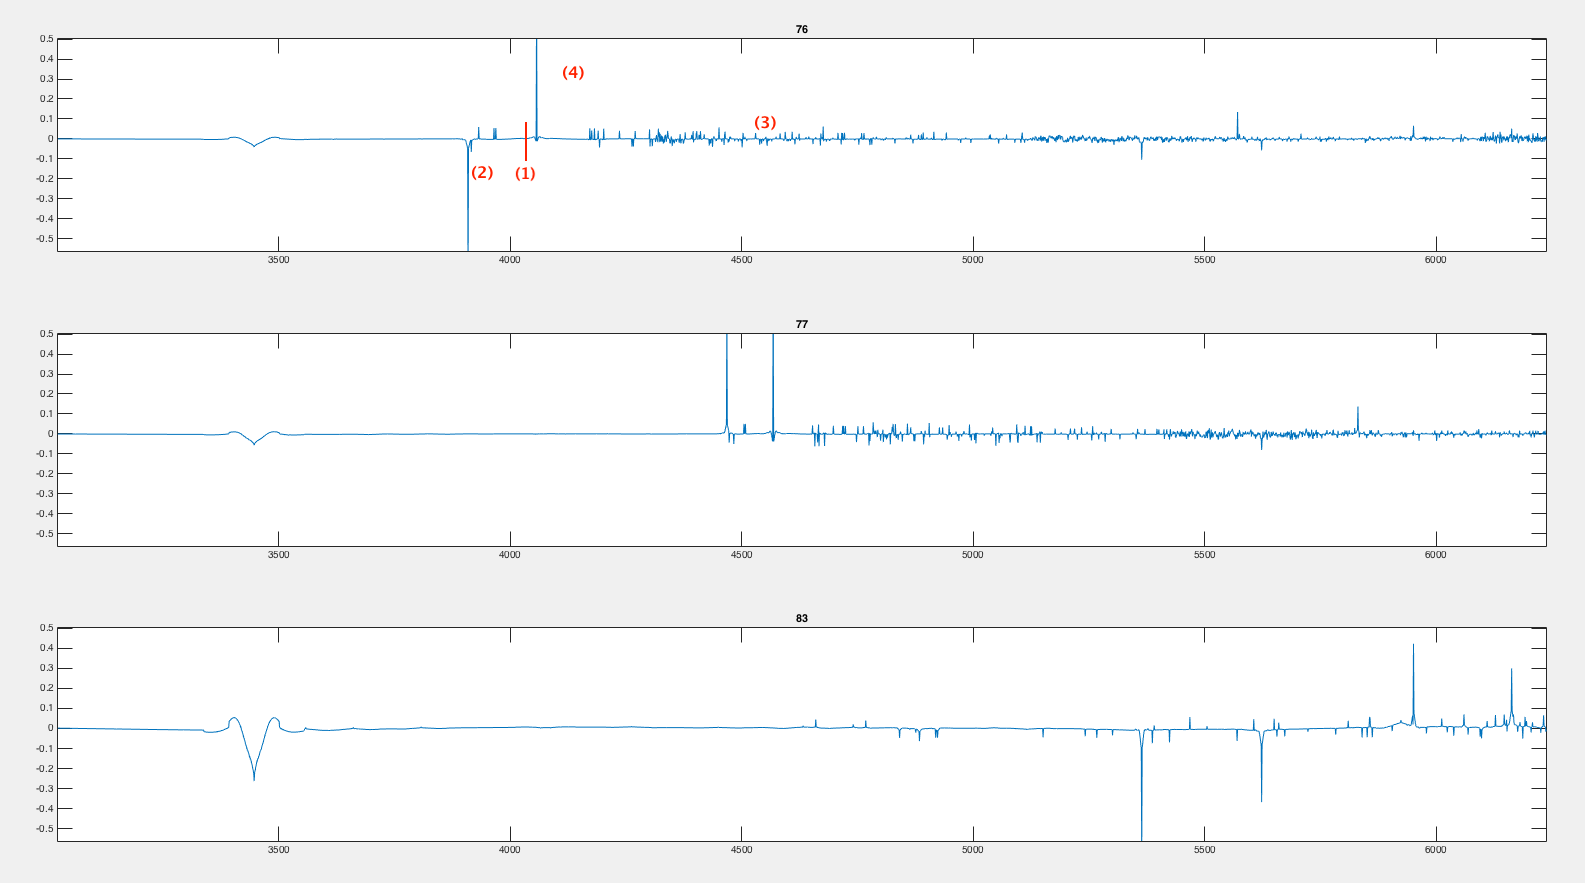
\includegraphics[scale = 0.3]{Sections/Implementation/Odeon/images/incorrectRIR/RIR_76_incorrect_edit.png}
				\caption{Initial \ac{RIR} output with receiver 5cm above sound source}
				\label{incorrectRIR}
			\end{figure}

			%Show Height Test Images

			%Show new RIRs with correct timings

		\subsubsection{RIR Locations}
			%How many RIRs and where?

			%Inaccuracies due to distance

			%Keep them anyway
	
\end{document}